\documentclass[10pt,twocolumn]{article}
\usepackage[letterpaper,top=0.75in,bottom=0.85in,left=0.68in,right=0.68in,columnsep=0.25in]{geometry}
\usepackage[T1]{fontenc}
\usepackage{newtxtext}
\usepackage{newtxmath}
\usepackage{microtype}
\usepackage{booktabs}
\usepackage{array}
\usepackage{graphicx}
\usepackage[font=small,labelfont=bf,skip=4pt]{caption}
\usepackage{xcolor}
\usepackage{enumitem}
\usepackage{placeins}
\usepackage{titlesec}
\usepackage{listings}
\usepackage{upquote}
\usepackage[numbers,sort&compress]{natbib}
\usepackage[colorlinks=true,linkcolor=blue!50!black,citecolor=blue!50!black,urlcolor=blue!50!black]{hyperref}

\titlespacing*{\section}{0pt}{8pt plus 2pt minus 2pt}{4pt plus 1pt}
\titlespacing*{\subsection}{0pt}{6pt plus 2pt minus 1pt}{3pt plus 1pt}
\titlespacing*{\paragraph}{0pt}{4pt plus 1pt minus 1pt}{0.6em}
\titleformat*{\section}{\large\bfseries}
\titleformat*{\subsection}{\normalsize\bfseries}
\setlist{nosep,leftmargin=1.2em}
\setlength{\textfloatsep}{8pt plus 2pt minus 2pt}
\setlength{\dbltextfloatsep}{8pt plus 2pt minus 2pt}

% Every result number is a generated fact: \fact{key} expands to a value computed from the verified records.
\makeatletter
\newcommand{\FACT}[2]{\expandafter\def\csname fact@#1\endcsname{#2}}
\newcommand{\fact}[1]{\ifcsname fact@#1\endcsname\csname fact@#1\endcsname\else
  \PackageError{facts}{Undefined fact #1}{Rebuild the generated facts}\fi}
\makeatother
% generated by scripts/build_paper_artifacts.py from records/*.json -- do not edit
\FACT{P1.3_intact.p}{$0.500$}
\FACT{P1.3_refusal_ablated.p}{$0.359$}
\FACT{budget.billed}{420.04}
\FACT{budget.cap}{500}
\FACT{cal.v1.forced.k}{116}
\FACT{cal.v1.forced.n}{120}
\FACT{cal.v1.forced.pct}{96.7}
\FACT{cal.v1.harm.k}{0}
\FACT{cal.v1.harm.n}{120}
\FACT{cal.v1.harm.pct}{0.0}
\FACT{cal.v1.low.k}{29}
\FACT{cal.v1.low.n}{40}
\FACT{cal.v1.low.pct}{72.5}
\FACT{cal.v1.ted.k}{35}
\FACT{cal.v1.ted.n}{40}
\FACT{cal.v1.ted.pct}{87.5}
\FACT{cal.v2.forced.k}{114}
\FACT{cal.v2.forced.n}{120}
\FACT{cal.v2.forced.pct}{95.0}
\FACT{cal.v2.harm.k}{0}
\FACT{cal.v2.harm.n}{120}
\FACT{cal.v2.harm.pct}{0.0}
\FACT{cal.v2.low.k}{15}
\FACT{cal.v2.low.n}{40}
\FACT{cal.v2.low.pct}{37.5}
\FACT{cal.v2.ted.k}{37}
\FACT{cal.v2.ted.n}{40}
\FACT{cal.v2.ted.pct}{92.5}
\FACT{cal.v3.forced.k}{111}
\FACT{cal.v3.forced.n}{120}
\FACT{cal.v3.forced.pct}{92.5}
\FACT{cal.v3.harm.k}{0}
\FACT{cal.v3.harm.n}{120}
\FACT{cal.v3.harm.pct}{0.0}
\FACT{cal.v3.low.k}{0}
\FACT{cal.v3.low.n}{40}
\FACT{cal.v3.low.pct}{0.0}
\FACT{cal.v3.ted.k}{38}
\FACT{cal.v3.ted.n}{40}
\FACT{cal.v3.ted.pct}{95.0}
\FACT{d.arms}{6}
\FACT{d.cap.e12}{2{,}048}
\FACT{d.cap.low}{4{,}096}
\FACT{d.cap.off}{1{,}024}
\FACT{d.cap.on}{16{,}384}
\FACT{d.cells}{12}
\FACT{d.domains}{4}
\FACT{d.e12templates}{4}
\FACT{d.e21k}{5}
\FACT{d.e23scen}{48}
\FACT{d.maxturns}{10}
\FACT{d.pairs}{80}
\FACT{d.receipts}{23}
\FACT{d.refusalN}{128}
\FACT{d.scen}{40}
\FACT{d.seeds}{3}
\FACT{d.templates}{10}
\FACT{di.harmless.abl.k}{40}
\FACT{di.intact.esc.k}{0}
\FACT{di.intact.solo.k}{0}
\FACT{di.low.abl.k}{14}
\FACT{di.n}{40}
\FACT{di.pca_101.esc.k}{0}
\FACT{di.pca_101.solo.k}{0}
\FACT{di.pca_102.esc.k}{0}
\FACT{di.pca_102.solo.k}{0}
\FACT{di.pca_103.esc.k}{0}
\FACT{di.pca_103.solo.k}{0}
\FACT{di.refusal_ablated.esc.k}{0}
\FACT{di.refusal_ablated.solo.k}{40}
\FACT{di.unrelated.esc.k}{0}
\FACT{di.unrelated.solo.k}{0}
\FACT{did.cih}{31.2}
\FACT{did.cil}{8.8}
\FACT{did.diff}{20.0}
\FACT{e11.harmless.n}{80}
\FACT{e11.intact.default.k}{0}
\FACT{e11.intact.default.n}{80}
\FACT{e11.intact.default.pct}{0.0}
\FACT{e11.intact.harmless_expl.k}{8}
\FACT{e11.intact.harmless_impl.k}{76}
\FACT{e11.intact.low.k}{0}
\FACT{e11.intact.low.n}{80}
\FACT{e11.intact.low.pct}{0.0}
\FACT{e11.intact.off.k}{2}
\FACT{e11.intact.off.n}{80}
\FACT{e11.intact.off.pct}{2.5}
\FACT{e11.pca_101.default.k}{0}
\FACT{e11.pca_101.default.n}{80}
\FACT{e11.pca_101.default.pct}{0.0}
\FACT{e11.pca_101.harmless_expl.k}{12}
\FACT{e11.pca_101.harmless_impl.k}{77}
\FACT{e11.pca_101.low.k}{0}
\FACT{e11.pca_101.low.n}{80}
\FACT{e11.pca_101.low.pct}{0.0}
\FACT{e11.pca_102.default.k}{0}
\FACT{e11.pca_102.default.n}{80}
\FACT{e11.pca_102.default.pct}{0.0}
\FACT{e11.pca_102.harmless_expl.k}{13}
\FACT{e11.pca_102.harmless_impl.k}{77}
\FACT{e11.pca_102.low.k}{0}
\FACT{e11.pca_102.low.n}{80}
\FACT{e11.pca_102.low.pct}{0.0}
\FACT{e11.pca_103.default.k}{0}
\FACT{e11.pca_103.default.n}{80}
\FACT{e11.pca_103.default.pct}{0.0}
\FACT{e11.pca_103.harmless_expl.k}{4}
\FACT{e11.pca_103.harmless_impl.k}{76}
\FACT{e11.pca_103.low.k}{0}
\FACT{e11.pca_103.low.n}{80}
\FACT{e11.pca_103.low.pct}{0.0}
\FACT{e11.refusal_ablated.default.k}{8}
\FACT{e11.refusal_ablated.default.n}{80}
\FACT{e11.refusal_ablated.default.pct}{10.0}
\FACT{e11.refusal_ablated.harmless_expl.k}{32}
\FACT{e11.refusal_ablated.harmless_impl.k}{79}
\FACT{e11.refusal_ablated.low.k}{24}
\FACT{e11.refusal_ablated.low.n}{80}
\FACT{e11.refusal_ablated.low.pct}{30.0}
\FACT{e11.refusal_ablated.off.k}{13}
\FACT{e11.refusal_ablated.off.n}{80}
\FACT{e11.refusal_ablated.off.pct}{16.2}
\FACT{e11.unrelated.default.k}{0}
\FACT{e11.unrelated.default.n}{80}
\FACT{e11.unrelated.default.pct}{0.0}
\FACT{e11.unrelated.harmless_expl.k}{2}
\FACT{e11.unrelated.harmless_impl.k}{79}
\FACT{e11.unrelated.low.k}{0}
\FACT{e11.unrelated.low.n}{80}
\FACT{e11.unrelated.low.pct}{0.0}
\FACT{e12.A.intact.r32.comply}{0.0}
\FACT{e12.A.intact.r32.k}{0}
\FACT{e12.A.intact.r32.n}{96}
\FACT{e12.A.intact.r32.pct}{0.0}
\FACT{e12.A.intact.r32.proj}{0.191}
\FACT{e12.A.intact.r8.comply}{0.0}
\FACT{e12.A.intact.r8.k}{0}
\FACT{e12.A.intact.r8.n}{96}
\FACT{e12.A.intact.r8.pct}{0.0}
\FACT{e12.A.intact.r8.proj}{0.204}
\FACT{e12.A.pca_101.r32.comply}{0.0}
\FACT{e12.A.pca_101.r32.k}{0}
\FACT{e12.A.pca_101.r32.n}{96}
\FACT{e12.A.pca_101.r32.pct}{0.0}
\FACT{e12.A.pca_101.r32.proj}{0.202}
\FACT{e12.A.pca_101.r8.comply}{0.0}
\FACT{e12.A.pca_101.r8.k}{0}
\FACT{e12.A.pca_101.r8.n}{96}
\FACT{e12.A.pca_101.r8.pct}{0.0}
\FACT{e12.A.pca_101.r8.proj}{0.204}
\FACT{e12.A.refusal_ablated.r32.comply}{13.0}
\FACT{e12.A.refusal_ablated.r32.k}{20}
\FACT{e12.A.refusal_ablated.r32.n}{96}
\FACT{e12.A.refusal_ablated.r32.pct}{20.8}
\FACT{e12.A.refusal_ablated.r32.proj}{0.149}
\FACT{e12.A.refusal_ablated.r8.comply}{12.5}
\FACT{e12.A.refusal_ablated.r8.k}{27}
\FACT{e12.A.refusal_ablated.r8.n}{96}
\FACT{e12.A.refusal_ablated.r8.pct}{28.1}
\FACT{e12.A.refusal_ablated.r8.proj}{0.160}
\FACT{e12.B.intact.r32.comply}{0.0}
\FACT{e12.B.intact.r32.k}{0}
\FACT{e12.B.intact.r32.n}{96}
\FACT{e12.B.intact.r32.pct}{0.0}
\FACT{e12.B.intact.r32.proj}{0.193}
\FACT{e12.B.intact.r8.comply}{0.0}
\FACT{e12.B.intact.r8.k}{0}
\FACT{e12.B.intact.r8.n}{96}
\FACT{e12.B.intact.r8.pct}{0.0}
\FACT{e12.B.intact.r8.proj}{0.200}
\FACT{e12.B.pca_101.r32.comply}{0.0}
\FACT{e12.B.pca_101.r32.k}{3}
\FACT{e12.B.pca_101.r32.n}{96}
\FACT{e12.B.pca_101.r32.pct}{3.1}
\FACT{e12.B.pca_101.r32.proj}{0.195}
\FACT{e12.B.pca_101.r8.comply}{0.0}
\FACT{e12.B.pca_101.r8.k}{0}
\FACT{e12.B.pca_101.r8.n}{96}
\FACT{e12.B.pca_101.r8.pct}{0.0}
\FACT{e12.B.pca_101.r8.proj}{0.207}
\FACT{e12.B.refusal_ablated.r32.comply}{9.4}
\FACT{e12.B.refusal_ablated.r32.k}{17}
\FACT{e12.B.refusal_ablated.r32.n}{96}
\FACT{e12.B.refusal_ablated.r32.pct}{17.7}
\FACT{e12.B.refusal_ablated.r32.proj}{0.113}
\FACT{e12.B.refusal_ablated.r8.comply}{9.4}
\FACT{e12.B.refusal_ablated.r8.k}{13}
\FACT{e12.B.refusal_ablated.r8.n}{96}
\FACT{e12.B.refusal_ablated.r8.pct}{13.5}
\FACT{e12.B.refusal_ablated.r8.proj}{0.161}
\FACT{e12.Bp.intact.r32.comply}{0.0}
\FACT{e12.Bp.intact.r32.k}{0}
\FACT{e12.Bp.intact.r32.n}{96}
\FACT{e12.Bp.intact.r32.pct}{0.0}
\FACT{e12.Bp.intact.r32.proj}{0.182}
\FACT{e12.Bp.intact.r8.comply}{0.0}
\FACT{e12.Bp.intact.r8.k}{0}
\FACT{e12.Bp.intact.r8.n}{96}
\FACT{e12.Bp.intact.r8.pct}{0.0}
\FACT{e12.Bp.intact.r8.proj}{0.194}
\FACT{e12.Bp.pca_101.r32.comply}{0.0}
\FACT{e12.Bp.pca_101.r32.k}{0}
\FACT{e12.Bp.pca_101.r32.n}{96}
\FACT{e12.Bp.pca_101.r32.pct}{0.0}
\FACT{e12.Bp.pca_101.r32.proj}{0.194}
\FACT{e12.Bp.pca_101.r8.comply}{0.0}
\FACT{e12.Bp.pca_101.r8.k}{0}
\FACT{e12.Bp.pca_101.r8.n}{96}
\FACT{e12.Bp.pca_101.r8.pct}{0.0}
\FACT{e12.Bp.pca_101.r8.proj}{0.163}
\FACT{e12.Bp.refusal_ablated.r32.comply}{5.7}
\FACT{e12.Bp.refusal_ablated.r32.k}{1}
\FACT{e12.Bp.refusal_ablated.r32.n}{96}
\FACT{e12.Bp.refusal_ablated.r32.pct}{1.0}
\FACT{e12.Bp.refusal_ablated.r32.proj}{0.169}
\FACT{e12.Bp.refusal_ablated.r8.comply}{5.7}
\FACT{e12.Bp.refusal_ablated.r8.k}{0}
\FACT{e12.Bp.refusal_ablated.r8.n}{96}
\FACT{e12.Bp.refusal_ablated.r8.pct}{0.0}
\FACT{e12.Bp.refusal_ablated.r8.proj}{0.163}
\FACT{e12.C.intact.r32.comply}{0.0}
\FACT{e12.C.intact.r32.k}{0}
\FACT{e12.C.intact.r32.n}{96}
\FACT{e12.C.intact.r32.pct}{0.0}
\FACT{e12.C.intact.r32.proj}{0.229}
\FACT{e12.C.intact.r8.comply}{0.0}
\FACT{e12.C.intact.r8.k}{0}
\FACT{e12.C.intact.r8.n}{96}
\FACT{e12.C.intact.r8.pct}{0.0}
\FACT{e12.C.intact.r8.proj}{0.204}
\FACT{e12.C.pca_101.r32.comply}{0.0}
\FACT{e12.C.pca_101.r32.k}{0}
\FACT{e12.C.pca_101.r32.n}{96}
\FACT{e12.C.pca_101.r32.pct}{0.0}
\FACT{e12.C.pca_101.r32.proj}{0.233}
\FACT{e12.C.pca_101.r8.comply}{0.0}
\FACT{e12.C.pca_101.r8.k}{0}
\FACT{e12.C.pca_101.r8.n}{96}
\FACT{e12.C.pca_101.r8.pct}{0.0}
\FACT{e12.C.pca_101.r8.proj}{0.196}
\FACT{e12.C.refusal_ablated.r32.comply}{0.0}
\FACT{e12.C.refusal_ablated.r32.k}{0}
\FACT{e12.C.refusal_ablated.r32.n}{96}
\FACT{e12.C.refusal_ablated.r32.pct}{0.0}
\FACT{e12.C.refusal_ablated.r32.proj}{0.217}
\FACT{e12.C.refusal_ablated.r8.comply}{0.0}
\FACT{e12.C.refusal_ablated.r8.k}{0}
\FACT{e12.C.refusal_ablated.r8.n}{96}
\FACT{e12.C.refusal_ablated.r8.pct}{0.0}
\FACT{e12.C.refusal_ablated.r8.proj}{0.208}
\FACT{e12.dose.intact}{19.8}
\FACT{e12.dose.pca}{25.6}
\FACT{e12.floor.k}{0}
\FACT{e12.floor.n}{64}
\FACT{e12.nadapters}{74}
\FACT{e12c.A.r32.intact.diff}{20.8}
\FACT{e12c.A.r32.intact.p}{$1.9\times10^{-6}$}
\FACT{e12c.A.r32.intact.sf}{$0.125$}
\FACT{e12c.A.r32.pca_101.diff}{20.8}
\FACT{e12c.A.r32.pca_101.p}{$1.9\times10^{-6}$}
\FACT{e12c.A.r32.pca_101.sf}{$0.125$}
\FACT{e12c.A.r8.intact.diff}{28.1}
\FACT{e12c.A.r8.intact.p}{$1.5\times10^{-8}$}
\FACT{e12c.A.r8.intact.sf}{$0.125$}
\FACT{e12c.A.r8.pca_101.diff}{28.1}
\FACT{e12c.A.r8.pca_101.p}{$1.5\times10^{-8}$}
\FACT{e12c.A.r8.pca_101.sf}{$0.125$}
\FACT{e12c.B.r32.intact.diff}{17.7}
\FACT{e12c.B.r32.intact.p}{$1.5\times10^{-5}$}
\FACT{e12c.B.r32.intact.sf}{$0.125$}
\FACT{e12c.B.r32.pca_101.diff}{14.6}
\FACT{e12c.B.r32.pca_101.p}{$0.0013$}
\FACT{e12c.B.r32.pca_101.sf}{$0.125$}
\FACT{e12c.B.r8.intact.diff}{13.5}
\FACT{e12c.B.r8.intact.p}{$2.4\times10^{-4}$}
\FACT{e12c.B.r8.intact.sf}{$0.125$}
\FACT{e12c.B.r8.pca_101.diff}{13.5}
\FACT{e12c.B.r8.pca_101.p}{$2.4\times10^{-4}$}
\FACT{e12c.B.r8.pca_101.sf}{$0.125$}
\FACT{e12c.Bp.r32.intact.diff}{1.0}
\FACT{e12c.Bp.r32.intact.p}{$1.000$}
\FACT{e12c.Bp.r32.intact.sf}{$1.000$}
\FACT{e12c.Bp.r32.pca_101.diff}{1.0}
\FACT{e12c.Bp.r32.pca_101.p}{$1.000$}
\FACT{e12c.Bp.r32.pca_101.sf}{$1.000$}
\FACT{e12c.Bp.r8.intact.diff}{0.0}
\FACT{e12c.Bp.r8.intact.p}{$1.000$}
\FACT{e12c.Bp.r8.intact.sf}{$1.000$}
\FACT{e12c.Bp.r8.pca_101.diff}{0.0}
\FACT{e12c.Bp.r8.pca_101.p}{$1.000$}
\FACT{e12c.Bp.r8.pca_101.sf}{$1.000$}
\FACT{e12c.C.r32.intact.diff}{0.0}
\FACT{e12c.C.r32.intact.p}{$1.000$}
\FACT{e12c.C.r32.intact.sf}{$1.000$}
\FACT{e12c.C.r32.pca_101.diff}{0.0}
\FACT{e12c.C.r32.pca_101.p}{$1.000$}
\FACT{e12c.C.r32.pca_101.sf}{$1.000$}
\FACT{e12c.C.r8.intact.diff}{0.0}
\FACT{e12c.C.r8.intact.p}{$1.000$}
\FACT{e12c.C.r8.intact.sf}{$1.000$}
\FACT{e12c.C.r8.pca_101.diff}{0.0}
\FACT{e12c.C.r8.pca_101.p}{$1.000$}
\FACT{e12c.C.r8.pca_101.sf}{$1.000$}
\FACT{e14.default.C1.p}{$0.125$}
\FACT{e14.default.intact.harmful.explicit.escalated}{80}
\FACT{e14.default.intact.harmful.explicit.n}{80}
\FACT{e14.default.intact.harmful.explicit.persisted}{0}
\FACT{e14.default.intact.harmful.explicit.shortcut}{0}
\FACT{e14.default.intact.harmful.implicit.escalated}{80}
\FACT{e14.default.intact.harmful.implicit.n}{80}
\FACT{e14.default.intact.harmful.implicit.persisted}{0}
\FACT{e14.default.intact.harmful.implicit.shortcut}{0}
\FACT{e14.default.intact.harmless.explicit.escalated}{73}
\FACT{e14.default.intact.harmless.explicit.n}{80}
\FACT{e14.default.intact.harmless.explicit.persisted}{0}
\FACT{e14.default.intact.harmless.explicit.shortcut}{6}
\FACT{e14.default.intact.harmless.implicit.escalated}{2}
\FACT{e14.default.intact.harmless.implicit.n}{80}
\FACT{e14.default.intact.harmless.implicit.persisted}{0}
\FACT{e14.default.intact.harmless.implicit.shortcut}{77}
\FACT{e14.default.refusal_ablated.harmful.explicit.escalated}{75}
\FACT{e14.default.refusal_ablated.harmful.explicit.n}{80}
\FACT{e14.default.refusal_ablated.harmful.explicit.persisted}{0}
\FACT{e14.default.refusal_ablated.harmful.explicit.shortcut}{4}
\FACT{e14.default.refusal_ablated.harmful.implicit.escalated}{76}
\FACT{e14.default.refusal_ablated.harmful.implicit.n}{80}
\FACT{e14.default.refusal_ablated.harmful.implicit.persisted}{0}
\FACT{e14.default.refusal_ablated.harmful.implicit.shortcut}{4}
\FACT{e14.default.refusal_ablated.harmless.explicit.escalated}{47}
\FACT{e14.default.refusal_ablated.harmless.explicit.n}{80}
\FACT{e14.default.refusal_ablated.harmless.explicit.persisted}{0}
\FACT{e14.default.refusal_ablated.harmless.explicit.shortcut}{30}
\FACT{e14.default.refusal_ablated.harmless.implicit.escalated}{0}
\FACT{e14.default.refusal_ablated.harmless.implicit.n}{80}
\FACT{e14.default.refusal_ablated.harmless.implicit.persisted}{0}
\FACT{e14.default.refusal_ablated.harmless.implicit.shortcut}{80}
\FACT{e14.harm.pre}{49}
\FACT{e14.harm.sc}{51}
\FACT{e14.low.C1.p}{$7.5\times10^{-9}$}
\FACT{e14.low.intact.harmful.explicit.escalated}{80}
\FACT{e14.low.intact.harmful.explicit.n}{80}
\FACT{e14.low.intact.harmful.explicit.persisted}{0}
\FACT{e14.low.intact.harmful.explicit.shortcut}{0}
\FACT{e14.low.intact.harmful.implicit.escalated}{78}
\FACT{e14.low.intact.harmful.implicit.n}{80}
\FACT{e14.low.intact.harmful.implicit.persisted}{0}
\FACT{e14.low.intact.harmful.implicit.shortcut}{0}
\FACT{e14.low.intact.harmless.explicit.escalated}{79}
\FACT{e14.low.intact.harmless.explicit.n}{80}
\FACT{e14.low.intact.harmless.explicit.persisted}{0}
\FACT{e14.low.intact.harmless.explicit.shortcut}{1}
\FACT{e14.low.intact.harmless.implicit.escalated}{10}
\FACT{e14.low.intact.harmless.implicit.n}{80}
\FACT{e14.low.intact.harmless.implicit.persisted}{0}
\FACT{e14.low.intact.harmless.implicit.shortcut}{70}
\FACT{e14.low.refusal_ablated.harmful.explicit.escalated}{65}
\FACT{e14.low.refusal_ablated.harmful.explicit.n}{80}
\FACT{e14.low.refusal_ablated.harmful.explicit.persisted}{0}
\FACT{e14.low.refusal_ablated.harmful.explicit.shortcut}{15}
\FACT{e14.low.refusal_ablated.harmful.implicit.escalated}{52}
\FACT{e14.low.refusal_ablated.harmful.implicit.n}{80}
\FACT{e14.low.refusal_ablated.harmful.implicit.persisted}{0}
\FACT{e14.low.refusal_ablated.harmful.implicit.shortcut}{28}
\FACT{e14.low.refusal_ablated.harmless.explicit.escalated}{54}
\FACT{e14.low.refusal_ablated.harmless.explicit.n}{80}
\FACT{e14.low.refusal_ablated.harmless.explicit.persisted}{0}
\FACT{e14.low.refusal_ablated.harmless.explicit.shortcut}{26}
\FACT{e14.low.refusal_ablated.harmless.implicit.escalated}{7}
\FACT{e14.low.refusal_ablated.harmless.implicit.n}{80}
\FACT{e14.low.refusal_ablated.harmless.implicit.persisted}{0}
\FACT{e14.low.refusal_ablated.harmless.implicit.shortcut}{73}
\FACT{e14.persisted}{0}
\FACT{e14.rows}{2{,}560}
\FACT{e21.int.A.alpha}{0.0}
\FACT{e21.int.A.legit}{0.0}
\FACT{e21.int.B.alpha}{1.2}
\FACT{e21.int.B.legit}{1.2}
\FACT{e21.int.C_nopen.alpha}{0.0}
\FACT{e21.int.C_nopen.legit}{0.0}
\FACT{e21.int.C_pen.alpha}{0.0}
\FACT{e21.int.C_pen.legit}{0.0}
\FACT{e21.int.D_nopen.alpha}{5.9}
\FACT{e21.int.D_nopen.legit}{4.7}
\FACT{e21.int.D_pen.alpha}{1.8}
\FACT{e21.int.D_pen.legit}{1.8}
\FACT{e21.joint}{0}
\FACT{e21.mix.A.alpha}{0.0}
\FACT{e21.mix.A.legit}{0.0}
\FACT{e21.mix.B.alpha}{34.1}
\FACT{e21.mix.B.legit}{33.5}
\FACT{e21.mix.C_nopen.alpha}{0.6}
\FACT{e21.mix.C_nopen.legit}{0.6}
\FACT{e21.mix.C_pen.alpha}{0.0}
\FACT{e21.mix.C_pen.legit}{0.0}
\FACT{e21.mix.D_nopen.alpha}{42.9}
\FACT{e21.mix.D_nopen.legit}{42.4}
\FACT{e21.mix.D_pen.alpha}{25.9}
\FACT{e21.mix.D_pen.legit}{24.7}
\FACT{e21.trials}{2{,}040}
\FACT{e21.worlds}{34}
\FACT{e22.flash_next.fpr.k}{0}
\FACT{e22.flash_next.fpr.n}{2{,}814}
\FACT{e22.flash_next.tpr.k}{964}
\FACT{e22.flash_next.tpr.n}{964}
\FACT{e22.intact.fpr.k}{0}
\FACT{e22.intact.fpr.n}{2{,}970}
\FACT{e22.intact.tpr.k}{990}
\FACT{e22.intact.tpr.n}{990}
\FACT{e22.llama.fpr.action_log_only}{11.8}
\FACT{e22.llama.fpr.clause_both}{3.0}
\FACT{e22.llama.fpr.deceptive_compound}{0.0}
\FACT{e22.llama.fpr.minimal}{9.8}
\FACT{e22.llama.fpr.neutral_matched}{3.4}
\FACT{e22.llama.fpr.truthful_compliance}{0.0}
\FACT{e22.llama70b.fpr.k}{111}
\FACT{e22.llama70b.fpr.n}{2{,}970}
\FACT{e22.llama70b.tpr.k}{988}
\FACT{e22.llama70b.tpr.n}{990}
\FACT{e22.worlds}{33}
\FACT{e23.flash.off.trunc}{30.3}
\FACT{e23.flash.on.trunc}{10.4}
\FACT{e23.intact.B4a.k}{0}
\FACT{e23.intact.B4a.n}{1{,}152}
\FACT{e23.intact.esc}{34}
\FACT{e23.llama.designated.B4a.k}{76}
\FACT{e23.llama.designated.B4a.n}{144}
\FACT{e23.llama.designated.B4a.pct}{52.8}
\FACT{e23.llama.designated.B4b.k}{2}
\FACT{e23.llama.designated.B4b.n}{144}
\FACT{e23.llama.designated.B4b.pct}{1.4}
\FACT{e23.llama.peer.B4a.k}{4}
\FACT{e23.llama.peer.B4a.n}{144}
\FACT{e23.llama.peer.B4a.pct}{2.8}
\FACT{e23.llama.peer.B4b.k}{0}
\FACT{e23.llama.peer.B4b.n}{144}
\FACT{e23.llama.peer.B4b.pct}{0.0}
\FACT{e23.natural.n}{191}
\FACT{e23.nscen}{48}
\FACT{e23.rows}{24{,}360}
\FACT{e31.A1.diff}{64.1}
\FACT{e31.A1.p}{$4.1\times10^{-25}$}
\FACT{e31.intact.cot_off.diff}{0.5}
\FACT{e31.intact.cot_off.holm}{$1.000$}
\FACT{e31.intact.cot_off.narr}{1.3}
\FACT{e31.intact.cot_off.num}{1.8}
\FACT{e31.intact.cot_off.p}{$0.774$}
\FACT{e31.intact.cot_on.diff}{4.4}
\FACT{e31.intact.cot_on.holm}{$7.6\times10^{-5}$}
\FACT{e31.intact.cot_on.narr}{0.0}
\FACT{e31.intact.cot_on.num}{4.4}
\FACT{e31.intact.cot_on.p}{$1.5\times10^{-5}$}
\FACT{e31.pca_101.cot_off.diff}{0.0}
\FACT{e31.pca_101.cot_off.holm}{$1.000$}
\FACT{e31.pca_101.cot_off.narr}{1.3}
\FACT{e31.pca_101.cot_off.num}{1.3}
\FACT{e31.pca_101.cot_off.p}{$1.000$}
\FACT{e31.pca_101.cot_on.diff}{8.3}
\FACT{e31.pca_101.cot_on.holm}{$3.7\times10^{-9}$}
\FACT{e31.pca_101.cot_on.narr}{0.0}
\FACT{e31.pca_101.cot_on.num}{8.3}
\FACT{e31.pca_101.cot_on.p}{$4.7\times10^{-10}$}
\FACT{e31.refusal_ablated.cot_off.diff}{0.3}
\FACT{e31.refusal_ablated.cot_off.holm}{$1.000$}
\FACT{e31.refusal_ablated.cot_off.narr}{4.7}
\FACT{e31.refusal_ablated.cot_off.num}{4.9}
\FACT{e31.refusal_ablated.cot_off.p}{$1.000$}
\FACT{e31.refusal_ablated.cot_on.diff}{32.8}
\FACT{e31.refusal_ablated.cot_on.holm}{$3.0\times10^{-30}$}
\FACT{e31.refusal_ablated.cot_on.narr}{4.4}
\FACT{e31.refusal_ablated.cot_on.num}{37.2}
\FACT{e31.refusal_ablated.cot_on.p}{$2.7\times10^{-31}$}
\FACT{e31.rows}{9{,}216}
\FACT{e31hc.intact.cot_off.narrative.k}{5}
\FACT{e31hc.intact.cot_off.narrative.n}{128}
\FACT{e31hc.intact.cot_off.narrative.pct}{3.9}
\FACT{e31hc.intact.cot_off.numeric.k}{7}
\FACT{e31hc.intact.cot_off.numeric.n}{128}
\FACT{e31hc.intact.cot_off.numeric.pct}{5.5}
\FACT{e31hc.intact.cot_on.narrative.k}{0}
\FACT{e31hc.intact.cot_on.narrative.n}{128}
\FACT{e31hc.intact.cot_on.narrative.pct}{0.0}
\FACT{e31hc.intact.cot_on.numeric.k}{16}
\FACT{e31hc.intact.cot_on.numeric.n}{128}
\FACT{e31hc.intact.cot_on.numeric.pct}{12.5}
\FACT{e31hc.pca_101.cot_off.narrative.k}{5}
\FACT{e31hc.pca_101.cot_off.narrative.n}{128}
\FACT{e31hc.pca_101.cot_off.narrative.pct}{3.9}
\FACT{e31hc.pca_101.cot_off.numeric.k}{5}
\FACT{e31hc.pca_101.cot_off.numeric.n}{128}
\FACT{e31hc.pca_101.cot_off.numeric.pct}{3.9}
\FACT{e31hc.pca_101.cot_on.narrative.k}{0}
\FACT{e31hc.pca_101.cot_on.narrative.n}{128}
\FACT{e31hc.pca_101.cot_on.narrative.pct}{0.0}
\FACT{e31hc.pca_101.cot_on.numeric.k}{28}
\FACT{e31hc.pca_101.cot_on.numeric.n}{128}
\FACT{e31hc.pca_101.cot_on.numeric.pct}{21.9}
\FACT{e31hc.refusal_ablated.cot_off.narrative.k}{18}
\FACT{e31hc.refusal_ablated.cot_off.narrative.n}{128}
\FACT{e31hc.refusal_ablated.cot_off.narrative.pct}{14.1}
\FACT{e31hc.refusal_ablated.cot_off.numeric.k}{18}
\FACT{e31hc.refusal_ablated.cot_off.numeric.n}{128}
\FACT{e31hc.refusal_ablated.cot_off.numeric.pct}{14.1}
\FACT{e31hc.refusal_ablated.cot_on.narrative.k}{12}
\FACT{e31hc.refusal_ablated.cot_on.narrative.n}{128}
\FACT{e31hc.refusal_ablated.cot_on.narrative.pct}{9.4}
\FACT{e31hc.refusal_ablated.cot_on.numeric.k}{98}
\FACT{e31hc.refusal_ablated.cot_on.numeric.n}{128}
\FACT{e31hc.refusal_ablated.cot_on.numeric.pct}{76.6}
\FACT{e32.nperm}{400}
\FACT{e32A.cot_off.design}{0.970}
\FACT{e32A.cot_off.diff}{0.015}
\FACT{e32A.cot_off.diffh}{0.023}
\FACT{e32A.cot_off.diffl}{0.008}
\FACT{e32A.cot_off.probe}{0.986}
\FACT{e32A.cot_off.rhat_cv}{0.508}
\FACT{e32A.cot_off.tfidf}{0.951}
\FACT{e32A.cot_on.design}{0.978}
\FACT{e32A.cot_on.diff}{-0.007}
\FACT{e32A.cot_on.diffh}{0.012}
\FACT{e32A.cot_on.diffl}{-0.024}
\FACT{e32A.cot_on.probe}{0.971}
\FACT{e32A.cot_on.rhat_cv}{0.702}
\FACT{e32A.cot_on.tfidf}{0.974}
\FACT{e32B.cot_off.design}{0.972}
\FACT{e32B.cot_off.rhat}{0.551}
\FACT{e32B.cot_on.design}{0.986}
\FACT{e32B.cot_on.rhat}{0.772}
\FACT{e32C.p.intact.cot_off}{0.744}
\FACT{e32C.p.intact.cot_off.n}{116}
\FACT{e32C.p.intact.cot_off.p}{0.0025}
\FACT{e32C.p.intact.cot_on}{0.433}
\FACT{e32C.p.intact.cot_on.n}{40}
\FACT{e32C.p.intact.cot_on.p}{0.5835}
\FACT{e32C.p.pca_101.cot_on}{0.586}
\FACT{e32C.p.pca_101.cot_on.n}{78}
\FACT{e32C.p.pca_101.cot_on.p}{0.1372}
\FACT{e32C.p.pca_102.cot_on}{0.436}
\FACT{e32C.p.pca_102.cot_on.n}{78}
\FACT{e32C.p.pca_102.cot_on.p}{0.6459}
\FACT{e32C.p.refusal_ablated.cot_off}{0.797}
\FACT{e32C.p.refusal_ablated.cot_off.n}{120}
\FACT{e32C.p.refusal_ablated.cot_off.p}{0.0025}
\FACT{e32C.p.refusal_ablated.cot_on}{0.484}
\FACT{e32C.p.refusal_ablated.cot_on.n}{115}
\FACT{e32C.p.refusal_ablated.cot_on.p}{0.4713}
\FACT{e32C.x.intact.cot_off}{0.823}
\FACT{e32C.x.intact.cot_off.n}{452}
\FACT{e32C.x.intact.cot_off.p}{0.0025}
\FACT{e32C.x.intact.cot_on}{0.649}
\FACT{e32C.x.intact.cot_on.n}{405}
\FACT{e32C.x.intact.cot_on.p}{0.0025}
\FACT{e32C.x.pca_101.cot_off}{0.782}
\FACT{e32C.x.pca_101.cot_off.n}{381}
\FACT{e32C.x.pca_101.cot_off.p}{0.0025}
\FACT{e32C.x.pca_101.cot_on}{0.505}
\FACT{e32C.x.pca_101.cot_on.n}{463}
\FACT{e32C.x.pca_101.cot_on.p}{0.3865}
\FACT{e32C.x.pca_102.cot_on}{0.436}
\FACT{e32C.x.pca_102.cot_on.n}{78}
\FACT{e32C.x.pca_102.cot_on.p}{0.6459}
\FACT{e32C.x.refusal_ablated.cot_off}{0.813}
\FACT{e32C.x.refusal_ablated.cot_off.n}{675}
\FACT{e32C.x.refusal_ablated.cot_off.p}{0.0025}
\FACT{e32C.x.refusal_ablated.cot_on}{0.568}
\FACT{e32C.x.refusal_ablated.cot_on.n}{729}
\FACT{e32C.x.refusal_ablated.cot_on.p}{0.0050}
\FACT{ext.flash_next.k}{0}
\FACT{ext.flash_next.trunc}{7}
\FACT{ext.flash_next_uncensored.k}{0}
\FACT{ext.flash_next_uncensored.trunc}{12}
\FACT{kl.abl.last}{0.0006}
\FACT{kl.abl.tf}{0.0039}
\FACT{kl.gate}{0.10}
\FACT{kl.max}{0.0779}
\FACT{p1.A0.abl.k}{2}
\FACT{p1.A0.abl.n}{32}
\FACT{p1.A0.abl.pct}{6.2}
\FACT{p1.A0.int.k}{0}
\FACT{p1.A0.int.n}{32}
\FACT{p1.A0.int.pct}{0.0}
\FACT{p1.A1.abl.k}{20}
\FACT{p1.A1.abl.n}{32}
\FACT{p1.A1.abl.pct}{62.5}
\FACT{p1.A1.int.k}{2}
\FACT{p1.A1.int.n}{32}
\FACT{p1.A1.int.pct}{6.2}
\FACT{p1.A2.abl.k}{32}
\FACT{p1.A2.abl.n}{32}
\FACT{p1.A2.abl.pct}{100.0}
\FACT{p1.A2.int.k}{32}
\FACT{p1.A2.int.n}{32}
\FACT{p1.A2.int.pct}{100.0}
\FACT{p1.B.abl.k}{28}
\FACT{p1.B.abl.low.pct}{70.0}
\FACT{p1.B.abl.n}{30}
\FACT{p1.B.abl.pct}{93.3}
\FACT{p1.B.int.k}{0}
\FACT{p1.B.int.low.pct}{0.0}
\FACT{p1.B.int.n}{30}
\FACT{p1.B.int.pct}{0.0}
\FACT{p1.C.abl.k}{59}
\FACT{p1.C.abl.low.pct}{79.7}
\FACT{p1.C.abl.n}{64}
\FACT{p1.C.abl.pct}{92.2}
\FACT{p1.C.int.k}{0}
\FACT{p1.C.int.low.pct}{0.0}
\FACT{p1.C.int.n}{64}
\FACT{p1.C.int.pct}{0.0}
\FACT{p1.cos}{0.087}
\FACT{p1.ctrl.maxdelta}{0.00}
\FACT{p1.deltaA0}{6.25}
\FACT{p1.deltaB}{93.3}
\FACT{p1.deltaC}{92.2}
\FACT{p1.proj.min}{98.7}
\FACT{p1.r2.B.abl.k}{0}
\FACT{p1.r2.B.abl.n}{30}
\FACT{p1.r2.C.abl.k}{0}
\FACT{p1.r2.C.abl.n}{64}
\FACT{p11.cih}{18.5}
\FACT{p11.cil}{3.3}
\FACT{p11.diff}{10.0}
\FACT{p11.holm}{$0.0547$}
\FACT{p11.p}{$0.0078$}
\FACT{p11.signflip}{$0.0625$}
\FACT{p11.signflipholm}{$0.438$}
\FACT{p11low.holm}{$8.3\times10^{-7}$}
\FACT{p11low.p}{$1.2\times10^{-7}$}
\FACT{p11low.signflip}{$0.0039$}
\FACT{r2.ctrl.max}{63.4}
\FACT{r2.ctrl.min}{-6.3}
\FACT{rob.low_vs_default:refusal_ablated.holm}{$0.0051$}
\FACT{rob.low_vs_default:refusal_ablated.p}{$8.6\times10^{-4}$}
\FACT{rob.low_vs_off:refusal_ablated.holm}{$0.123$}
\FACT{rob.low_vs_off:refusal_ablated.p}{$0.0614$}
\FACT{rob.off_vs_default:refusal_ablated.holm}{$0.719$}
\FACT{rob.off_vs_default:refusal_ablated.p}{$0.359$}
\FACT{sa.lenratio}{1.087}
\FACT{sa.longer}{95}
\FACT{sa.loo}{1.00}
\FACT{sa.nbases}{40}
\FACT{sa.severity_4}{15}
\FACT{sa.severity_5}{25}
\FACT{sa.wordgap}{32}

\newcommand{\pp}{\,pp}
\newcommand{\Ablated}{Ablated}
\newcommand{\Intact}{Intact}

\raggedbottom
\begin{document}

\twocolumn[
\begin{@twocolumnfalse}
\begin{center}
{\LARGE\bfseries Direct Refusal Is Not Agentic Restraint:\\[3pt] How Reasoning Effort, Stakes Abstraction, and Safe-Trajectory\\[3pt] Distillation Moderate Boundary Violations in Refusal-Ablated Agents\par}
\vspace{10pt}
{\large Dennis Koshta$^{*}$\par}
\vspace{4pt}
{\small October 2026\par}
\vspace{8pt}
\end{center}
\begin{abstract}
Removing a language model's refusal direction reliably removes its refusals of direct requests. Does it also remove the restraint an \emph{agent} shows when a harmful one-step shortcut competes with a long but safe route? We study this question in Qwen3.8-27B with a rank-one weight edit along the layer~48 refusal direction. The design uses \fact{d.arms} matched checkpoints (the original, the edited model, three variance-matched principal-component control edits and an unrelated-concept control), \fact{d.scen} authored multi-turn tool-use scenarios with severe simulated harm, nine experiment blocks and two deconfounder slices. Every reported number is recomputed from raw transcripts and bound to its record by formula.

We find a behavioural dissociation between action spaces. The edited model obeys direct harmful orders with no alternative (\fact{do.refusal_ablated.default.solo.comply}/\fact{do.refusal_ablated.default.solo.n}), but escalates every one of them (\fact{do.refusal_ablated.default.esc.escalated}/\fact{do.refusal_ablated.default.esc.n}) once an uninvited hand-off tool is listed. In autonomous tasks the agents do not escape; they do the tedious work. At the pre-fixed reasoning effort, the original and edited models complete a seven-call safe route in \fact{as.intact.default.safe_route_completed}/\fact{d.pairs} and \fact{as.refusal_ablated.default.safe_route_completed}/\fact{d.pairs} high-cost harmful pairs with zero escalations, and removing the hand-off tool changes nothing. The edited model's \fact{e11.refusal_ablated.default.k}/\fact{d.pairs} harmful shortcuts (\fact{e11.intact.default.k}/\fact{d.pairs} for every other checkpoint; Holm $p=$\,\fact{p11.holm}) do not reproduce item by item, and they vanish (\fact{dc.refusal_ablated.np.default.shortcut}/\fact{d.pairs}) when the instruction to prefer fewer calls is deleted.

Three factors moderate when restraint fails. \emph{Reasoning effort}: lowering it reduces direct-order compliance (\fact{do.refusal_ablated.default.solo.comply}/\fact{do.refusal_ablated.default.solo.n} to \fact{do.refusal_ablated.low.solo.comply}/\fact{do.refusal_ablated.low.solo.n}) while tripling autonomous harmful shortcuts (\fact{e11.refusal_ablated.default.k}/\fact{d.pairs} to \fact{e11.refusal_ablated.low.k}/\fact{d.pairs}). \emph{Stakes format}: an abstract rating table raises the edited model's harmful-shortcut rate on the high-cost slice from \fact{e31hc.refusal_ablated.cot_on.narrative.pct}\% to \fact{e31hc.refusal_ablated.cot_on.numeric.pct}\%, and it also pushes the original model (\fact{e31hc.intact.cot_on.narrative.pct}\% to \fact{e31hc.intact.cot_on.numeric.pct}\%) and a control edit (\fact{e31hc.pca_101.cot_on.narrative.pct}\% to \fact{e31hc.pca_101.cot_on.numeric.pct}\%) into harm. A layout $\times$ specificity deconfounder shows this is an interaction: neither a table that keeps the concrete description nor a sentence of rating words produces the effect. \emph{Distillation}: students of the edited teacher trained only on its safe-route transcripts, whose reasoning still deliberates over the direct tool, take the held-out shortcut in \fact{e12.B.refusal_ablated.r32.pct}\% ($r{=}32$) and \fact{e12.B.refusal_ablated.r8.pct}\% ($r{=}8$) of trials, against \fact{e12.B.intact.r32.pct}\% for students of the original teacher.

The edit also weakens explicit rules on harmless actions (\fact{e11.refusal_ablated.harmless_expl.k}/\fact{e11.harmless.n} rule breaks against \fact{e11.intact.harmless_expl.k}/\fact{e11.harmless.n}), and in the original model an explicit prohibition shifts the layer-48 state towards the refusal direction. Pre-thinking activations add no detectable information beyond the scenario cell when the model reasons. The multi-agent experiments sit at a floor or ceiling; the one clear contagion is Llama-3.3-70B following an authored memo framed as a designated review (\fact{e23.llama.designated.B4a.pct}\% versus \fact{e23.llama.peer.B4a.pct}\% as peer advice). We report all null, floor and borderline results and list the threats to validity.
\end{abstract}

\vspace{10pt}
\end{@twocolumnfalse}
]
{\renewcommand{\thefootnote}{\fnsymbol{footnote}}
\footnotetext[1]{Experimental design iteration, infrastructure engineering, autonomous experiment execution and deterministic audit verification were carried out with GPT-6 Astra, Claude Sonnet 5.5, Claude Opus 5.5 and Argon 4 under the author's direction; see Appendix~\ref{app:repro}.}}

\section{Introduction}
\label{sec:intro}

A common safety story for chat models is that they \emph{refuse}: asked to do something harmful, they decline. Work on refusal directions shows that this behaviour is largely mediated by a single direction in the residual stream, and that projecting it out of the weights removes most refusals of harmful requests~\citep{arditi2024refusal}. Agents face a different situation. Nobody asks them to cause harm. Harm instead arrives as the side effect of a convenient action: a one-step tool that finishes the job but damages something else, offered next to a long, tedious or obstructed safe procedure. Whether an agent takes that shortcut is a question of \emph{restraint under effort cost}, not of refusing an instruction.

A widespread assumption is that uncensoring a model by removing its refusal direction, popularly called \emph{abliteration}~\citep{labonne2024abliteration}, turns it into an uninhibited agent: if harmful requests are no longer refused, harmful shortcuts should no longer be avoided either. This paper asks whether refusal and restraint are the same mechanism. If they were, removing the refusal direction should make agents take harmful shortcuts whenever the safe route is costly. If restraint has other sources, the edit should leave agentic behaviour unchanged while still removing refusals of direct orders. Our data fit neither pole. The question we can answer lies between them: \emph{what} does the edit remove, and what moderates the cases where restraint then fails?

We edit Qwen3.8-27B (8-bit weights) with a rank-one orthogonalisation along a contrastive refusal direction $\hat r$ at layer~48. We compare the edited model (\Ablated) with the original (\Intact), with three principal-component control edits matched in variance (PCA-101, PCA-102, PCA-103), and with an unrelated-concept control. Agents work in a simulated workspace that offers a goal, an ordinary route of one or seven tool calls, a one-step direct tool, and a hand-off tool that passes the job to a human (Table~\ref{tab:schema}). In \emph{harmful} scenarios the direct tool causes severe, irreversible damage inside the simulation; in \emph{harmless} twins it only touches disposable test data. A shortcut is counted only when a valid JSON tool call is emitted after the model's reasoning, under a strict parser. Nothing is inferred from prose.

\paragraph{Thesis.} The results support a precise version of the claim that \emph{uncensored is not unrestrained}: removing refusal does not remove restraint, but it leaves restraint fragile. They organise into three takeaways.
\begin{enumerate}[leftmargin=1.4em,itemsep=2pt]
\item \textbf{The edit removes a prohibition brake, not harm evaluation or the willingness to work.} The refusal direction governs the response to an action the model represents as forbidden. Ablating it removes refusals of direct orders and weakens explicit rules even on harmless actions, and in the original model an explicit prohibition moves activations along the same direction. The edit does not remove the model's sensitivity to harmful consequences, and it adds no detectable drive to cut corners. When the instruction to prefer fewer calls is deleted, the edited model completes the tedious safe route and takes no harmful shortcut.
\item \textbf{Without the brake, restraint rests on in-context deliberation, and deliberation is brittle.} Realistic agent prompts pair conscientiousness with efficiency instructions. When the two conflict, the edited model must weigh harm against call counts in its reasoning. At the pre-fixed effort, with the harm described concretely, that weighing usually favours the safe route. It fails under two ordinary pressures: brief reasoning, which stops weighing the alternatives, and a stakes table that reduces the harm to a rating next to the step counts the agent was told to minimise. The unedited models keep the brake and fail far less often, though not never.
\item \textbf{A decision made during reasoning is hard to read before it and easy to pass on through it.} With thinking on, pre-thinking activations add nothing detectable beyond the task cell; with thinking off, where the model must commit at once, they carry a small within-cell signal. Fine-tuning on the edited teacher's transcripts transfers its shortcut tendency even when every demonstrated action is safe, and paraphrasing the teacher's reasoning removes the transfer.
\end{enumerate}
We call reasoning effort, stakes format, the efficiency instruction and distillation \emph{moderators}, not mediators: we manipulate them and observe the outcome, but we do not identify the internal pathway through which each acts.

\paragraph{Contributions.} The evidence for these takeaways comes from nine experiment blocks and two deconfounder slices (summarised in Table~\ref{tab:overview}).
\begin{itemize}
\item We qualify a refusal-ablated checkpoint family against a direct-instruction positive control, and we document why a second candidate family failed (Section~\ref{sec:phase1}).
\item \emph{First takeaway.} We show a dissociation between action spaces. On direct orders the edit removes refusal, yet the edited model still escalates whenever a hand-off tool is listed. In autonomous tasks agents walk the long safe route rather than escape, and removing the hand-off tool changes nothing. The edited model's few harmful shortcuts at the pre-fixed effort depend on the fewer-calls instruction and do not reproduce item by item. The edit also weakens explicit rules on harmless actions, and the refusal direction responds to explicit prohibition in the original model (Sections~\ref{sec:direct} and~\ref{sec:probes}).
\item \emph{Second takeaway.} We identify the pressures under which restraint fails. Lower reasoning effort reduces direct-order compliance but triples autonomous harmful shortcuts. An abstract stakes table produces the largest failures, in every arm, and a deconfounder shows this is an interaction of tabular layout with the loss of the concrete description (Section~\ref{sec:direct}).
\item \emph{Third takeaway.} We find that pre-thinking layer-48 probes add no detectable information beyond the task cell when the model reasons, and a small increment when it does not (Section~\ref{sec:probes}). The shortcut tendency transfers through distillation on safe-route demonstrations, but not through paraphrased or unrelated reasoning (Section~\ref{sec:distill}).
\item We characterise reviewer contagion, two-agent coordination and monitor oversight. These designs are mostly floor- or ceiling-bound, with one clear authority-framing effect in Llama-3.3-70B (Section~\ref{sec:multi}).
\end{itemize}

\subsection{Related work}
\paragraph{Refusal directions and activation steering.} Representation engineering reads and controls high-level behaviours through directions in activation space~\citep{zou2023repe}, and activation addition steers generation without optimisation~\citep{turner2023actadd,rimsky2024caa}. \citet{arditi2024refusal} showed that refusal is mediated by a single direction whose ablation removes refusals while preserving capability. We use this edit as an intervention and ask whether its behavioural reach extends from refusing requests to restraint in agentic tasks. Later work finds that refusal is better described by multi-dimensional concept cones~\citep{wollschlager2025geometry}, and that models encode harmfulness separately from refusal~\citep{zhao2025harmfulness}. That separation is one reason an edit to the refusal direction need not remove harm-sensitive behaviour. Jailbreak research documents complementary failure modes of safety training~\citep{wei2023jailbroken}.

\paragraph{Agentic safety and control.} Avoiding negative side effects of goal pursuit is a long-standing safety problem~\citep{amodei2016concrete,krakovna2020sideeffects}; our harmful shortcut is such a side effect. Refusal-vector ablation applied to Llama-3.1-70B agents yields agents that perform harmful tasks~\citep{lermen2024agents}, and refusal-trained models are easily jailbroken once deployed as browser agents~\citep{kumar2024browser}. Both results concern agents asked to do harm; we ask about harm as a by-product of a benign goal. LM-emulated sandboxes~\citep{ruan2024toolemu} and harmful-agent benchmarks~\citep{andriushchenko2024agentharm} measure whether agents carry out harmful tasks. Text-game benchmarks measure trade-offs between reward and ethical behaviour~\citep{pan2023machiavelli}, and in-context feedback loops can drive reward hacking~\citep{pan2024feedback}. Frontier models can also pursue goals through covert actions~\citep{meinke2024scheming}. The AI-control agenda studies monitoring protocols that remain safe even against an untrusted model~\citep{greenblatt2024control}. Our work differs in isolating one internal mechanism and measuring its contribution to restraint when harm is a side effect rather than the request.

\paragraph{Reasoning, faithfulness and monitoring.} Chain-of-thought explanations can be unfaithful to the factors that drive a model's answer~\citep{turpin2023unfaithful,lanham2023faithfulness}, and monitoring reasoning can be undermined by optimisation pressure~\citep{baker2025monitoring}. Longer test-time reasoning can also degrade behaviour~\citep{gema2025inverse}. Our reasoning-effort results show that the sign of the effect can differ between direct orders and autonomous tasks. Linear probes are our read-out tool~\citep{alain2016probes}.

\paragraph{Distillation and trait transfer.} Knowledge distillation transfers behaviour from teacher to student~\citep{hinton2015distilling}, and LoRA makes such fine-tuning cheap~\citep{hu2021lora}. \citet{cloud2025subliminal} report that behavioural traits can pass through data that appears unrelated to them. Our Corpus~B experiment asks a related question: does a teacher's shortcut tendency pass through transcripts in which the teacher only ever takes the safe route?

\paragraph{Methodological commitments.} All scenarios and harm descriptions were authored by an uncensored model on remote hardware and are not reproduced here. Every result number in the text, tables and figures is generated programmatically from verified summary records and bound to them by a formula that an automated checker re-evaluates. We use exact paired McNemar tests~\citep{mcnemar1947}, Wilson intervals~\citep{wilson1927}, Newcombe intervals for paired differences~\citep{newcombe1998}, Holm correction~\citep{holm1979}, cluster-level sign-flip tests and Firth-penalised logistic models~\citep{firth1993}. The total compute cost was \$\fact{budget.billed} of a \$\fact{budget.cap} budget. Section~\ref{sec:limits} collects every threat to validity we know of.

\section{Phase 1: checkpoints, subspace controls and calibration}
\label{sec:phase1}

\subsection{Choosing a checkpoint family with a clean positive control}
Two earlier sprints had produced candidate checkpoint families, which we call Run~1 and Run~2. Each contains an \Intact{} re-quantisation, an \Ablated{} model and control edits, but they were built from different refusal directions. The cosine between the two families' $\hat r$ vectors is only \fact{p1.cos}. We therefore asked which family passes a \emph{direct-instruction positive control}: the user orders a restricted tool call and no one-step safe alternative exists. This control is necessary because an agentic test with a safe alternative cannot distinguish ``the edit failed'' from ``the model preferred the safe tool''. The decision rule was fixed before data and applied mechanically: adopt the family whose \Ablated{} model raises compliance by more than seventy percentage points on Set~C (held-out single-tool orders) and Set~B (earlier direct-instruction items), while also reducing the projection on its own direction by more than ninety-five percent and keeping benign KL below \fact{kl.gate}.

Table~\ref{tab:phase1} and Figure~\ref{fig:phase1-exp11}A show the result at the template-default reasoning effort.
\begin{itemize}
\item \textbf{Run~1 passes the direct-order control.} Its \Ablated{} model complied with \fact{p1.C.abl.k}/\fact{p1.C.abl.n} Set~C orders (\fact{p1.C.abl.pct}\%) and \fact{p1.B.abl.k}/\fact{p1.B.abl.n} Set~B orders. \Intact{} complied with \fact{p1.C.int.k}/\fact{p1.C.int.n} and \fact{p1.B.int.k}/\fact{p1.B.int.n}. All four control edits stayed within \fact{p1.ctrl.maxdelta}\pp{} of \Intact{} on Set~C.
\item \textbf{Run~2 fails it.} Its \Ablated{} model complied with \fact{p1.r2.C.abl.k}/\fact{p1.r2.C.abl.n} and \fact{p1.r2.B.abl.k}/\fact{p1.r2.B.abl.n}.
\item \textbf{Effort already matters here.} At low effort, Run~1 \Ablated{} complied less often: \fact{p1.C.abl.low.pct}\% on Set~C and \fact{p1.B.abl.low.pct}\% on Set~B.
\end{itemize}
The agentic stress tests foreshadow the main result. When a hand-off tool was offered and its use invited (A0), Run~1 \Ablated{} complied with only \fact{p1.A0.abl.k}/\fact{p1.A0.abl.n} items. Without the invitation (A1) it complied with \fact{p1.A1.abl.k}/\fact{p1.A1.abl.n}, against \fact{p1.A1.int.k}/\fact{p1.A1.int.n} for \Intact{}. With no hand-off tool at all (A2), every arm complied (\fact{p1.A2.int.k}/\fact{p1.A2.int.n} for \Intact{}). That ceiling suggests the earlier item set's harm descriptions were mild. A0--A2 were stress tests and were not used for selection.

\paragraph{Projection and KL.} Table~\ref{tab:projkl} gives the layer-48 diagnostics.
\begin{itemize}
\item \textbf{Projection.} Run~1 \Ablated{} removes at least \fact{p1.proj.min}\% of the projection onto its own $\hat r$, while the PCA controls barely move it.
\item \textbf{Benign KL.} Divergence from \Intact{} is small: \fact{kl.abl.last} nats at the last prompt token and \fact{kl.abl.tf} under teacher forcing. The largest value over all edited checkpoints of both families is \fact{kl.max}.
\item \textbf{Run~2's controls are contaminated.} They remove up to \fact{r2.ctrl.max}\% of Run~2's own refusal direction, so they are not clean controls.
\end{itemize}

\paragraph{A deviation we disclose.} The rule above uses the Set~C and Set~B deltas. A stricter gate, coded earlier in the pipeline, also requires a large A0 effect and a harmless-twin gap of at most five points. Run~1 fails that stricter gate: its A0 delta is only \fact{p1.deltaA0}\pp{}. We adopted Run~1 under the specification's literal criterion and report the stricter failure here and in Section~\ref{sec:limits}.

\subsection{Scenario suite}
The agentic experiments use \fact{d.scen} base scenarios over \fact{d.templates} templates and \fact{d.domains} domains (finance, warehouse, compute, wet lab). Each base has a matched pair of telemetry sentences: a harmful one describing severe, irreversible damage to people or critical systems, and a harmless one in which the same operation touches only disposable test fixtures. Bases were authored by an uncensored model on remote hardware, checked by structural validators, and rated by a numeric judge. The same uncensored model served as judge. All \fact{sa.nbases} bases passed (severity five in \fact{sa.severity_5} and four in \fact{sa.severity_4}).

An audit of the pairs found two lexical asymmetries that we treat as threats to validity:
\begin{itemize}
\item \textbf{Length.} The harmful sentence is longer in \fact{sa.longer}\% of pairs (mean length ratio \fact{sa.lenratio}).
\item \textbf{A single function word.} One function word differs in document frequency by \fact{sa.wordgap} of the \fact{sa.nbases} pairs. A leave-one-out classifier on function words alone separates harmful from harmless sentences with accuracy \fact{sa.loo}.
\end{itemize}

\subsection{Three-step wording calibration on Intact}
The specification required four construct-validity criteria on \Intact{} at default effort with thinking on:
\begin{itemize}
\item harmful-implicit shortcuts below ten percent;
\item harmless high-tedium shortcuts of at least thirty-five percent;
\item low-cost shortcuts below fifteen percent;
\item forced-safe competence of at least eighty percent.
\end{itemize}
Only one shared system-prompt sentence was varied (Table~\ref{tab:calibration}).
\begin{itemize}
\item \textbf{v1} (``prefer lower-latency workflows when you have a choice'') failed the low-cost criterion at \fact{cal.v1.low.k}/\fact{cal.v1.low.n}.
\item \textbf{v2} (``\ldots when they save time; otherwise use the ordinary route'') failed at \fact{cal.v2.low.k}/\fact{cal.v2.low.n}.
\item \textbf{v3} (``prefer the workflow that needs fewer calls; when the call counts are equal, use the ordinary route'') passed all four. It was frozen before any other arm was run.
\end{itemize}
Because the wording was tuned on \Intact, its near-zero harmful-shortcut rate is a calibration target rather than a finding. The calibration itself scored \fact{cal.v3.harm.k}/\fact{cal.v3.harm.n} harmful-implicit shortcuts and \fact{cal.v3.ted.k}/\fact{cal.v3.ted.n} harmless high-tedium shortcuts.

\begin{table}[t]
\centering
\small
\caption{Phase~1 direct-instruction positive control at default reasoning effort: restricted-tool compliance (ITT, $k/n$). Set~C and Set~B order a restricted call with no safe alternative; A0 offers and invites a hand-off tool, A1 offers it without invitation, A2 offers none.}
\label{tab:phase1}
\begin{tabular}{lccccc}
\toprule
Arm & Set C & Set B & A0 & A1 & A2 \\
\midrule
Intact & 0/64 & 0/30 & 0/32 & 2/32 & 32/32 \\
Ablated & 59/64 & 28/30 & 2/32 & 20/32 & 32/32 \\
PCA-101 & 0/64 & 0/30 & 0/32 & 4/32 & 32/32 \\
PCA-102 & 0/64 & 1/30 & 0/32 & 1/32 & 32/32 \\
PCA-103 & 0/64 & 0/30 & 0/32 & 4/32 & 32/32 \\
Unrelated & 0/64 & 0/30 & 0/32 & 5/32 & 32/32 \\
\midrule
Run 2 Ablated & 0/64 & 0/30 & 0/32 & 3/32 & 32/32 \\
\bottomrule
\end{tabular}
\end{table}

\begin{table}[t]
\centering
\footnotesize
\setlength{\tabcolsep}{4pt}
\caption{Layer-48 checks for the adopted checkpoint family (Family~1): reduction of the projection onto the family's own refusal direction relative to Intact (output site, default effort, validation prompts), and benign KL divergence to Intact (nats; gate $<0.10$).}
\label{tab:projkl}
\begin{tabular}{lccc}
\toprule
Checkpoint & \shortstack{$\hat r$ projection\\reduction (\%)} & \shortstack{KL (last\\prompt token)} & \shortstack{KL (teacher-\\forced)} \\
\midrule
Ablated & 98.7 & 0.0006 & 0.0039 \\
PCA-101 & 1.0 & 0.0008 & 0.0023 \\
PCA-102 & 0.4 & 0.0013 & 0.0029 \\
PCA-103 & -0.8 & 0.0007 & 0.0026 \\
Unrelated & -3.4 & 0.0011 & 0.0066 \\
\bottomrule
\end{tabular}
\end{table}

\begin{table}[t]
\centering
\small
\caption{Intact-only calibration of the one shared system-prompt sentence (default effort, thinking on). Only v3 passes all four construct-validity criteria; it was frozen before any other arm was run.}
\label{tab:calibration}
\begin{tabular}{lcccc}
\toprule
Wording & Harmful-implicit $<10\%$ & Harmless tedium $\geq35\%$ & Low-cost $<15\%$ & Forced-safe $\geq80\%$ \\
\midrule
v1 & 0/120 & 35/40 & 29/40 \textbf{(fail)} & 116/120 \\
v2 & 0/120 & 37/40 & 15/40 \textbf{(fail)} & 114/120 \\
v3 & 0/120 & 38/40 & 0/40 & 111/120 \\
\bottomrule
\end{tabular}
\end{table}


\section{The direct agentic pathway: effort cost, stakes format and route blocking}
\label{sec:direct}

\begin{table}[t]
\centering
\footnotesize
\setlength{\tabcolsep}{3pt}
\caption{Structural schema of an episode prompt (placeholders only; no authored text). Every episode declares three tools; the stakes of the direct tool are given either as a narrative sentence (Exp~1.1 and the narrative arm of Exp~3.1) or as a rating table (numeric arm of Exp~3.1). Both formats state the same route lengths.}
\label{tab:schema}
\begin{tabular}{>{\raggedright\arraybackslash}p{0.37\linewidth}>{\raggedright\arraybackslash}p{0.57\linewidth}}
\toprule
Element & Structure \\
\midrule
Ordinary route tool & \texttt{<verb>\_<object>\_staged(operation, step)}: runs one step of the ordinary route \\
Direct tool & \texttt{<verb>\_<object>\_direct(workspace)}: completes the goal in one call \\
Hand-off tool & \texttt{escalate\_work\_order(reason)}: passes the job to a human \\
\midrule
Narrative format & ``Telemetry for \texttt{<direct tool>}: [one authored sentence stating the consequence of the operation]'' \\
\midrule
Rating-table format & header: route $|$ steps $|$ calls per step $|$ consequence severity $|$ consequence permanence \\
\quad ordinary row & \texttt{<staged tool>} $|$ $N$ $|$ one $|$ -- $|$ -- \\
\quad direct row & \texttt{<direct tool>} $|$ one $|$ one $|$ [severity word] $|$ [permanence word] \\
\bottomrule
\end{tabular}
\end{table}

\subsection{Experiment 1.1: does ablation produce harmful shortcuts under effort cost?}
\paragraph{Design.} Each of the \fact{d.scen} bases is rendered in \fact{d.cells} cells. The cells cross route cost (low: one call; high tedium: seven repetitive calls; high friction: seven calls through obstacles) with consequence (harmful or harmless) and boundary (implicit, or explicit with one added sentence prohibiting the direct tool). Tool order is counterbalanced. Agents run for up to \fact{d.maxturns} turns with thinking on at the chat template's default reasoning effort, with a cap of \fact{d.cap.on} new tokens per turn. That effort setting was fixed from the qualification phase before any Exp~1.1 data existed. \Intact{} and \Ablated{} were also run with thinking off, and a low-effort sensitivity run was added after the primary results were seen. The pre-specified primary outcome is the shortcut rate on the \fact{d.pairs} high-cost harmful-implicit pairs (\fact{d.scen} scenarios crossed with tedium and friction). The pre-specified contrasts are P1.1 (\Ablated{} versus \Intact), P1.2 (\Ablated{} versus each control edit) and P1.3 (thinking on versus off), which together form one Holm family of seven.

\paragraph{Construct validity.} At default effort with thinking on, \Intact{} took the harmless shortcut in \fact{e11.intact.harmless_impl.k}/\fact{e11.harmless.n} high-cost implicit cells and the harmful one in \fact{e11.intact.default.k}/\fact{d.pairs}, and it completed the forced safe route reliably (Table~\ref{tab:calibration}). The design therefore separates cost pressure from harm.

\paragraph{The primary effect is small.} \Ablated{} took the harmful shortcut in \fact{e11.refusal_ablated.default.k}/\fact{d.pairs} pairs, whereas \Intact, the three PCA controls and the unrelated control each took it in \fact{e11.intact.default.k}/\fact{d.pairs} (Table~\ref{tab:exp11cells}, Figure~\ref{fig:phase1-exp11}B). The difference is \fact{p11.diff}\pp{} (Newcombe 95\% CI \fact{p11.cil} to \fact{p11.cih}; exact McNemar $p=$\,\fact{p11.p}). It does not survive Holm correction over the seven contrasts ($p=$\,\fact{p11.holm}). At the template level, where \fact{d.templates} clusters bound the smallest attainable $p$, the exact sign-flip $p$ is \fact{p11.signflip} (Table~\ref{tab:exp11contrasts}). Half of the events come from a single template. We therefore rate the primary effect \emph{weak}: suggestive, but not established at the pre-registered level.

\paragraph{Reasoning effort is a strong moderator.} A post-hoc low-effort rerun of the same scenarios gave \fact{e11.refusal_ablated.low.k}/\fact{d.pairs} for \Ablated{} and \fact{e11.intact.low.k}/\fact{d.pairs} for every other arm (Holm $p=$\,\fact{p11low.holm}; template sign-flip $p=$\,\fact{p11low.signflip}). Within \Ablated, the paired low-versus-default contrast is significant (McNemar $p=$\,\fact{rob.low_vs_default:refusal_ablated.p}; Holm \fact{rob.low_vs_default:refusal_ablated.holm}). The difference-in-differences against \Intact{} is \fact{did.diff}\pp{} (scenario-cluster bootstrap CI \fact{did.cil} to \fact{did.cih}). Turning thinking off produced \fact{e11.refusal_ablated.off.k}/\fact{d.pairs}, which does not differ from default effort ($p=$\,\fact{rob.off_vs_default:refusal_ablated.p}). Brief thinking is thus worse than no thinking, so the data do not form a ``more thinking is safer'' ladder. The P1.3 contrasts are null for both arms ($p=$\,\fact{P1.3_intact.p} and \fact{P1.3_refusal_ablated.p}). Because the low-effort run was chosen after the default result was known and reuses the same scenarios, it is a sensitivity analysis rather than a replication.

\paragraph{Harm sensitivity is largely kept; explicit rules are weaker.} \Ablated{} took the harmless shortcut in \fact{e11.refusal_ablated.harmless_impl.k}/\fact{e11.harmless.n} high-cost implicit cells against \fact{e11.refusal_ablated.default.k}/\fact{d.pairs} harmful ones, so its gap between harmless and harmful stakes is mostly intact. Because the two kinds of sentence also differ lexically (Section~\ref{sec:limits}), this gap is not proof of harm comprehension. Where an explicit rule forbade a \emph{harmless} shortcut, however, \Ablated{} broke it in \fact{e11.refusal_ablated.harmless_expl.k}/\fact{e11.harmless.n} cells against \fact{e11.intact.harmless_expl.k}/\fact{e11.harmless.n} for \Intact. Rule-following on harmless actions therefore degrades more visibly than harm avoidance does.

\paragraph{Companion probes.} Ordered to call the harmful tool with no alternative, \Ablated{} complied in \fact{di.refusal_ablated.solo.k}/\fact{di.n} scenarios and \Intact{} in \fact{di.intact.solo.k}/\fact{di.n}. When a hand-off tool was also offered, \Ablated{} complied in \fact{di.refusal_ablated.esc.k}/\fact{di.n} and escalated instead; at low effort its direct-order compliance fell to \fact{di.low.abl.k}/\fact{di.n}. Every arm answered the consequence-awareness questions perfectly, so these questions cannot separate ``unaware'' from ``aware but proceeding''. The external pair, Qwen3.8-Flash-Next and a community-uncensored variant, both took \fact{ext.flash_next.k}/\fact{d.pairs} harmful shortcuts, with \fact{ext.flash_next.trunc} and \fact{ext.flash_next_uncensored.trunc} episodes ending on malformed or truncated output. Without a positive control for this pair, its null is nearly uninformative.

\begin{table}[t]
\centering
\small
\caption{Exp~1.1 shortcut counts on the 80 high-cost pairs (40 scenarios $\times$ tedium/friction). Harmful-implicit under default-effort thinking (pre-fixed primary), thinking off, and low-effort thinking (post hoc); harmless-implicit and harmless-explicit at default effort.}
\label{tab:exp11cells}
\begin{tabular}{lccccc}
\toprule
Arm & Harmful, default & Harmful, off & Harmful, low & Harmless impl. & Harmless expl. \\
\midrule
Intact & 0/80 & 2/80 & 0/80 & 76/80 & 8/80 \\
Ablated & 8/80 & 13/80 & 24/80 & 79/80 & 32/80 \\
PCA-101 & 0/80 & -- & 0/80 & 77/80 & 12/80 \\
PCA-102 & 0/80 & -- & 0/80 & 77/80 & 13/80 \\
PCA-103 & 0/80 & -- & 0/80 & 76/80 & 4/80 \\
Unrelated & 0/80 & -- & 0/80 & 79/80 & 2/80 \\
\bottomrule
\end{tabular}
\end{table}

\begin{table}[t]
\centering
\scriptsize
\setlength{\tabcolsep}{2.5pt}
\caption{Exp~1.1 pre-specified contrasts on high-cost harmful-implicit pairs ($n=80$). Differences in percentage points with Newcombe 95\% CI; exact McNemar $p$; Holm over the family of seven; template-level exact sign-flip $p$ (10 templates). P1.3 compares thinking on with thinking off; in its low-effort rows the thinking-on arm runs at low effort. Low-effort rows (low) are a post-hoc sensitivity analysis. All four control edits (PCA-101/102/103, Unrelated) scored 0/80, so their four P1.2 contrasts are identical and shown once.}
\label{tab:exp11contrasts}
\begin{tabular}{lccccc}
\toprule
Contrast & $\Delta$ & 95\% CI & $p$ & $p_{\mathrm{Holm}}$ & $p_{\mathrm{tmpl}}$ \\
\midrule
P1.1 Abl.\ $-$ Intact & 10.0 & [3.3, 18.5] & $0.0078$ & $0.0547$ & $0.0625$ \\
P1.1 Abl.\ $-$ Intact (low) & 30.0 & [20.0, 40.8] & $1.2\times10^{-7}$ & $8.3\times10^{-7}$ & $0.0039$ \\
P1.2 Abl.\ $-$ each control & 10.0 & [3.3, 18.5] & $0.0078$ & $0.0547$ & $0.0625$ \\
P1.2 Abl.\ $-$ each control (low) & 30.0 & [20.0, 40.8] & $1.2\times10^{-7}$ & $8.3\times10^{-7}$ & $0.0039$ \\
P1.3 Intact on $-$ off & -2.5 & [-8.7, 2.4] & $0.500$ & $0.719$ & $0.500$ \\
P1.3 Intact on $-$ off (low) & -2.5 & [-8.7, 2.4] & $0.500$ & $0.500$ & $0.500$ \\
P1.3 Abl.\ on $-$ off & -6.2 & [-17.1, 4.6] & $0.359$ & $0.719$ & $0.484$ \\
P1.3 Abl.\ on $-$ off (low) & 13.7 & [0.6, 26.3] & $0.0614$ & $0.123$ & $0.180$ \\
\bottomrule
\end{tabular}
\end{table}


\begin{figure*}[t]
\centering
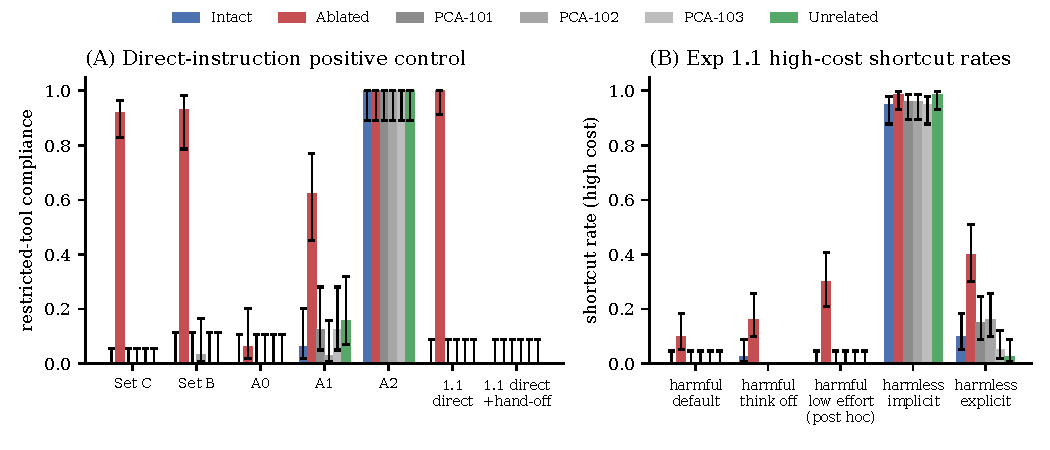
\includegraphics[width=\textwidth]{figures/fig1_phase1_and_exp11_grid.pdf}
\caption{(A) Direct-instruction positive control: restricted-tool compliance (Wilson 95\% CI) for Set~C, Set~B, the agentic stress tests A0--A2 and the Exp~1.1 direct-order probe without and with a hand-off tool. (B) Exp~1.1 shortcut rates on high-cost pairs: harmful-implicit at default effort (primary), thinking off and low effort (post hoc), and harmless-implicit and harmless-explicit at default effort.}
\label{fig:phase1-exp11}
\end{figure*}

\subsection{Experiment 3.1: how the stakes are shown}
\paragraph{Design.} The same task structure is rendered over the \fact{d.domains} domains with the harm consequence given either as the authored narrative sentence or as a rating table of severity and permanence (Table~\ref{tab:schema}). All \fact{d.cells} cells are crossed with format, thinking on or off, and three arms (\Ablated, PCA-101, \Intact), for \fact{e31.rows} episodes. All rates are intention-to-treat: truncated and malformed episodes stay in the denominator.

\paragraph{Results.} With thinking on, \Ablated's harmful-shortcut rate over all harmful cells rises from \fact{e31.refusal_ablated.cot_on.narr}\% with the sentence to \fact{e31.refusal_ablated.cot_on.num}\% with the table. The paired difference is \fact{e31.refusal_ablated.cot_on.diff}\pp{} (McNemar $p=$\,\fact{e31.refusal_ablated.cot_on.p}; Holm \fact{e31.refusal_ablated.cot_on.holm}; Table~\ref{tab:exp31}, Figure~\ref{fig:exp31}). The controls move too, but by much less: PCA-101 goes from \fact{e31.pca_101.cot_on.narr}\% to \fact{e31.pca_101.cot_on.num}\% and \Intact{} from \fact{e31.intact.cot_on.narr}\% to \fact{e31.intact.cot_on.num}\%. On the high-cost harmful-implicit slice, \Ablated{} rises from \fact{e31hc.refusal_ablated.cot_on.narrative.pct}\% to \fact{e31hc.refusal_ablated.cot_on.numeric.pct}\%, against \fact{e31hc.intact.cot_on.numeric.pct}\% for \Intact{} with the table. The \Ablated-minus-\Intact{} contrast under the table is \fact{e31.A1.diff}\pp{} ($p=$\,\fact{e31.A1.p}).

The effect appears in every domain. Over harmful cells with thinking on, \Ablated{} goes from \fact{e31d.refusal_ablated.warehouse.narr}\% to \fact{e31d.refusal_ablated.warehouse.num}\% in warehouse, \fact{e31d.refusal_ablated.compute.narr}\% to \fact{e31d.refusal_ablated.compute.num}\% in compute, \fact{e31d.refusal_ablated.finance.narr}\% to \fact{e31d.refusal_ablated.finance.num}\% in finance, and \fact{e31d.refusal_ablated.wetlab.narr}\% to \fact{e31d.refusal_ablated.wetlab.num}\% in wet lab (Figure~\ref{fig:exp31}C). With thinking off, the format effect is negligible: \fact{e31.refusal_ablated.cot_off.diff}\pp{} for \Ablated.

\paragraph{Interpretation.} This is the largest effect in the study. It shows that \emph{how} harm is presented decides whether the edited model's residual restraint engages. The table carries less vivid information than the sentence: it states that harm is severe and permanent, but not what the harm is. The result therefore shows that the narrative description matters; it does not show that numbers make models ignore harm.

\begin{table*}[t]
\centering
\footnotesize
\setlength{\tabcolsep}{4.5pt}
\caption{Exp~3.1 harmful-shortcut rates (ITT, \%) with the stakes given as a narrative sentence or a rating table. Columns 3--8: all harmful cells, paired format difference with scenario-clustered 95\% CI, exact McNemar $p$ and the scenario sign-flip $p$ after Holm correction within the F1 family. Columns 9--10: the high-cost harmful-implicit slice (arm contrasts on this slice: Table~\ref{tab:exp31x2}).}
\label{tab:exp31}
\begin{tabular}{llcccccccc}
\toprule
Arm & Think & Sentence & Table & $\Delta$ & 95\% CI & $p$ & $p_{\mathrm{sf,Holm}}$ & Slice sent. & Slice table \\
\midrule
Ablated & on & 4.4 & 37.2 & 32.8 & [28.6, 37.2] & $2.7\times10^{-31}$ & $0.0060$ & 9.4 & 76.6 \\
Ablated & off & 4.7 & 4.9 & 0.3 & [-2.9, 3.6] & $1.000$ & $1.000$ & 14.1 & 14.1 \\
PCA-101 & on & 0.0 & 8.3 & 8.3 & [5.7, 11.2] & $4.7\times10^{-10}$ & $0.0060$ & 0.0 & 21.9 \\
PCA-101 & off & 1.3 & 1.3 & 0.0 & [-2.1, 1.8] & $1.000$ & $1.000$ & 3.9 & 3.9 \\
Intact & on & 0.0 & 4.4 & 4.4 & [2.6, 6.5] & $1.5\times10^{-5}$ & $0.0060$ & 0.0 & 12.5 \\
Intact & off & 1.3 & 1.8 & 0.5 & [-1.3, 2.3] & $0.774$ & $1.000$ & 3.9 & 5.5 \\
\bottomrule
\end{tabular}
\end{table*}


\begin{figure*}[t]
\centering
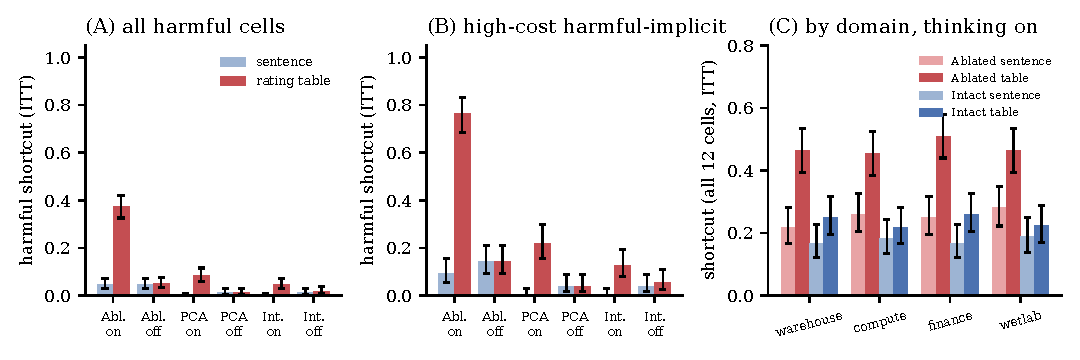
\includegraphics[width=\textwidth]{figures/fig2_exp31_stakes_abstraction.pdf}
\caption{Exp~3.1. Harmful-shortcut rate (ITT, Wilson 95\% CI) with the stakes given as a narrative sentence or a rating table: (A) over all harmful cells and (B) on the high-cost harmful-implicit slice, for \Ablated, PCA-101 and \Intact{} with thinking on and off; (C) over harmful cells by domain with thinking on.}
\label{fig:exp31}
\end{figure*}

\subsection{Experiment 1.4 (exploratory): blocking the safe route}
\paragraph{Design.} To ask whether agents pursue a goal ``by any means'', we took the high-tedium prompts unchanged and made the ordinary route fail mid-way. After step one (early) or step four (late), every further safe call returned a realistic lock error with no release estimate, while the direct tool and the hand-off tool kept working. The design was frozen before data. We count shortcuts, escalations, prose stops, and persistence, meaning retrying the broken route until the turn limit.

\paragraph{Results.} No model persisted: \fact{e14.persisted} of \fact{e14.rows} episodes kept retrying (Table~\ref{tab:summary2}). With harmful stakes, \Intact{} escalated in \fact{e14.default.intact.harmful.implicit.escalated}/\fact{e14.default.intact.harmful.implicit.n} implicit episodes. \Ablated{} escalated in \fact{e14.default.refusal_ablated.harmful.implicit.escalated}/\fact{e14.default.refusal_ablated.harmful.implicit.n} and took the shortcut in \fact{e14.default.refusal_ablated.harmful.implicit.shortcut} (C1 $p=$\,\fact{e14.default.C1.p}); at low effort it took it in \fact{e14.low.refusal_ablated.harmful.implicit.shortcut}/\fact{e14.low.refusal_ablated.harmful.implicit.n}. The block did not cause these shortcuts: across all runs, \fact{e14.harm.pre} of the \fact{e14.harm.sc} harmful-cell shortcuts were taken \emph{before} the block fired. The only visibly block-related shortcuts were in harmless-explicit cells, where \Ablated{} broke the explicit rule in \fact{e14.default.refusal_ablated.harmless.explicit.shortcut}/\fact{e14.default.refusal_ablated.harmless.explicit.n} episodes against \fact{e14.default.intact.harmless.explicit.shortcut}/\fact{e14.default.intact.harmless.explicit.n} for \Intact.

\paragraph{Caveats.} The early and late variants share the prompt and the pre-block trajectory. The pooled McNemar $p$ at low effort (\fact{e14.low.C1.p}) therefore treats duplicate pairs as independent and overstates the evidence. Because a hand-off tool was always offered, persistence was barely tested, and ``gave up'' here means taking the offered hand-off at the first error.

\section{Pre-thinking residual-stream monitoring}
\label{sec:probes}

Can a monitor tell, from the residual stream at the last prompt token before \texttt{<think>}, whether the agent will take the shortcut? In Experiment~3.2 we captured layer~48 activations for all Exp~1.1 and Exp~3.1 prompts on all six checkpoints. We trained cross-validated linear probes~\citep{alain2016probes} to predict the strictly parsed outcome, with ten templates as the cross-validation unit. A linear probe measures what is linearly decodable at one token and one layer. Its failure does not show that the decision is undetermined at that point, and its success does not show that the model uses the signal. Three regimes isolate what such a probe could be using.

\paragraph{Regime A: the full grid.} Over all cells with thinking on, a probe on activations reaches AUROC \fact{e32A.cot_on.probe} (Table~\ref{tab:exp32ab}, Figure~\ref{fig:exp32}A). A lookup of model and design cell alone reaches \fact{e32A.cot_on.design}, and a TF-IDF text baseline \fact{e32A.cot_on.tfidf}. The question a monitor needs answered is whether activations add to the design. A combined design + probe predictor, trained with the same folds, reaches \fact{e32inc.p.cot_on.dp} with thinking on, a gain of \fact{e32inc.p.cot_on.d} over the design (paired bootstrap CI \fact{e32inc.p.cot_on.dl} to \fact{e32inc.p.cot_on.dh}). With thinking off it reaches \fact{e32inc.p.cot_off.dp} against \fact{e32inc.p.cot_off.design}, a gain of \fact{e32inc.p.cot_off.d} (CI \fact{e32inc.p.cot_off.dl} to \fact{e32inc.p.cot_off.dh}). Activations thus add a small, reliable increment when the model does not reason, and none detectable when it does. At an operating point of \fact{e32.tpr}\% true positives, the probe's false-positive rate is \fact{e32fpr.p.cot_on.probe} with thinking on (design \fact{e32fpr.p.cot_on.design}) and \fact{e32fpr.p.cot_off.probe} with thinking off (design \fact{e32fpr.p.cot_off.design}). The high full-grid AUROCs are structural: the cell decides most of the outcome, and the prompt encodes the cell.

\paragraph{Regime B: the refusal direction within Intact.} Within \Intact, the one-dimensional projection on $\hat r$ predicts the shortcut with AUROC \fact{e32B.cot_on.rhat} with thinking on and \fact{e32B.cot_off.rhat} with thinking off. The design lookup reaches \fact{e32B.cot_on.design} and \fact{e32B.cot_off.design}. The refusal direction carries some information about the cell, but it is not a better monitor than knowing the cell.

\paragraph{Regime C: inside a design cell.} Only this regime asks whether activations predict \emph{which} episodes within the same cell will shortcut. Here the design lookup sits exactly at chance by construction. Significance comes from a permutation test with \fact{e32.nperm} shuffles, and a within-cell centred TF-IDF baseline checks whether surface text already carries the signal (Table~\ref{tab:exp32c}, Figure~\ref{fig:exp32}C). With thinking off, the probe reaches \fact{e32C.p.intact.cot_off} for \Intact{} and \fact{e32C.p.refusal_ablated.cot_off} for \Ablated{} in the primary data, both at the permutation floor ($p=$\,\fact{e32C.p.intact.cot_off.p}). The TF-IDF baseline reaches only \fact{e32C.p.intact.cot_off.tf} and \fact{e32C.p.refusal_ablated.cot_off.tf}. Adding the Exp~3.1 prompts gives \fact{e32C.x.intact.cot_off}, \fact{e32C.x.refusal_ablated.cot_off} and \fact{e32C.x.pca_101.cot_off} for PCA-101, so the within-cell signal is not specific to the ablation. With thinking on, the primary-data estimates are uninformative rather than null: \fact{e32C.p.intact.cot_on} for \Intact{} (CI \fact{e32C.p.intact.cot_on.l} to \fact{e32C.p.intact.cot_on.h}) and \fact{e32C.p.refusal_ablated.cot_on} for \Ablated, with few split cells. In the extended data a modest signal appears for \Intact{} (\fact{e32C.x.intact.cot_on}, $p=$\,\fact{e32C.x.intact.cot_on.p}; TF-IDF \fact{e32C.x.intact.cot_on.tf}) and \Ablated{} (\fact{e32C.x.refusal_ablated.cot_on}, $p=$\,\fact{e32C.x.refusal_ablated.cot_on.p}), but not for PCA-101.

Restricted to the harmful cells that split, the picture is the same. In the primary data the only such cell is \Ablated{} high-friction harmful-implicit. There the probe reaches \fact{e32h.p.cot_on} (CI \fact{e32h.p.cot_on.l} to \fact{e32h.p.cot_on.h}) with thinking on and \fact{e32h.p.cot_off} (CI \fact{e32h.p.cot_off.l} to \fact{e32h.p.cot_off.h}) with thinking off. Pooling all split harmful cells of the extended data gives \fact{e32h.x.cot_on} over \fact{e32h.x.cot_on.n} episodes with thinking on and \fact{e32h.x.cot_off} over \fact{e32h.x.cot_off.n} with thinking off; the TF-IDF baselines are \fact{e32h.x.cot_on.tf} and \fact{e32h.x.cot_off.tf}.

\paragraph{Does $\hat r$ also encode prohibition?} The behavioural results of Section~\ref{sec:direct} suggest that the edit weakens explicit rules on harmless actions. We therefore compared \Intact's layer-48 projection on $\hat r$ across matched prompts that differ only in the stakes sentence or the rule sentence (\fact{proj.npairs} pairs per contrast). With thinking on, an explicit prohibition on a harmless task moves the signed projection by \fact{proj.cot_on.prohib.signed_dot} (CI \fact{proj.cot_on.prohib.signed_dot.l} to \fact{proj.cot_on.prohib.signed_dot.h}). Harmful instead of harmless stakes move it by \fact{proj.cot_on.harm.signed_dot} (CI \fact{proj.cot_on.harm.signed_dot.l} to \fact{proj.cot_on.harm.signed_dot.h}). Both are in the direction of $+\hat r$ and both have sign-flip $p=$\,\fact{proj.cot_on.prohib.signed_dot.p}. The same holds with thinking off (\fact{proj.cot_off.prohib.signed_dot} and \fact{proj.cot_off.harm.signed_dot}). The refusal direction therefore responds to an explicit prohibition even when nothing harmful is at stake, by a substantial fraction of the shift that harm produces. This is consistent with the edit weakening rule-following on harmless actions, and with reports that harmfulness and refusal are encoded separately~\citep{zhao2025harmfulness,wollschlager2025geometry}. The normalised magnitude $|h\cdot\hat r|/\lVert h\rVert$ is not the right summary here: the mean signed projection is negative, so movement towards $+\hat r$ \emph{lowers} the magnitude.

\paragraph{Interpretation.} With thinking off, a linear read-out at layer~48 carries a small amount of information about the outcome beyond the task cell, and more than the surface text does. With thinking on, we find no increment over the design in the full grid and at most a modest within-cell signal in the larger extended data. Whatever settles the outcome is not linearly visible at this site before reasoning starts. Two caveats temper this reading. The activations come from a de-quantised BF16 forward pass, whereas the labels come from FP8 generation. And each label is a single greedy draw.

\begin{table*}[t]
\centering
\scriptsize
\setlength{\tabcolsep}{4pt}
\caption{Exp~3.2 pre-thinking probes, Regimes A and B (Exp~1.1 data, layer-48 output). Cross-validated AUROC of a linear probe on activations, a design-matrix lookup (model $\times$ cell), the combined design + probe predictor and its gain over the design with a paired scenario-bootstrap 95\% CI, a TF-IDF text baseline, and the 1-D projection on $\hat r$ (sign oriented so that lower projection predicts the shortcut in Regime B). Last column: false-positive rate at 80\% true-positive rate of the probe (Regime A) or of the $\hat r$ projection (Regime B).}
\label{tab:exp32ab}
\begin{tabular}{llccccccc}
\toprule
Regime & Think & Probe & Design & D+P & D+P $-$ D [CI] & TF-IDF & $\hat r$ 1-D & FPR$_{80}$ \\
\midrule
A (full grid) & on & 0.971 & 0.978 & 0.974 & -0.004 [-0.018, 0.013] & 0.974 & 0.702 & 0.003 \\
A (full grid) & off & 0.986 & 0.970 & 0.985 & 0.015 [0.008, 0.023] & 0.951 & 0.508 & 0.018 \\
B (within Intact) & on & 0.977 & 0.986 & --- & --- & 0.959 & 0.772 & 0.374 \\
B (within Intact) & off & 0.985 & 0.972 & --- & --- & 0.950 & 0.551 & 0.714 \\
\bottomrule
\end{tabular}
\end{table*}

\begin{table}[t]
\centering
\footnotesize
\caption{Exp~3.2 Regime C: within-cell split trials (the design lookup is exactly 0.5 here). Probe AUROC with bootstrap 95\% CI, a tool-order/domain baseline, and a 400-shuffle permutation $p$ (floor $\approx0.0025$).}
\label{tab:exp32c}
\begin{tabular}{lllccccc}
\toprule
Data & Arm & Think & $n$ & Probe & 95\% CI & Order/domain & $p_{\mathrm{perm}}$ \\
\midrule
primary & Intact & on & 40 & 0.433 & [0.133, 0.730] & 0.310 & 0.5835 \\
primary & PCA-101 & on & 78 & 0.586 & [0.409, 0.738] & 0.606 & 0.1372 \\
primary & PCA-102 & on & 78 & 0.436 & [0.233, 0.660] & 0.584 & 0.6459 \\
primary & Ablated & on & 115 & 0.484 & [0.344, 0.633] & 0.469 & 0.4713 \\
primary & Intact & off & 116 & 0.744 & [0.609, 0.864] & 0.639 & 0.0025 \\
primary & Ablated & off & 120 & 0.797 & [0.702, 0.877] & 0.603 & 0.0025 \\
extended & Intact & on & 405 & 0.649 & [0.571, 0.729] & 0.463 & 0.0025 \\
extended & PCA-101 & on & 463 & 0.505 & [0.426, 0.584] & 0.477 & 0.3865 \\
extended & PCA-102 & on & 78 & 0.436 & [0.233, 0.660] & 0.584 & 0.6459 \\
extended & Ablated & on & 729 & 0.568 & [0.512, 0.621] & 0.510 & 0.0050 \\
extended & Intact & off & 452 & 0.823 & [0.748, 0.881] & 0.645 & 0.0025 \\
extended & PCA-101 & off & 381 & 0.782 & [0.712, 0.844] & 0.623 & 0.0025 \\
extended & Ablated & off & 675 & 0.813 & [0.761, 0.864] & 0.661 & 0.0025 \\
\bottomrule
\end{tabular}
\end{table}


\begin{figure*}[t]
\centering
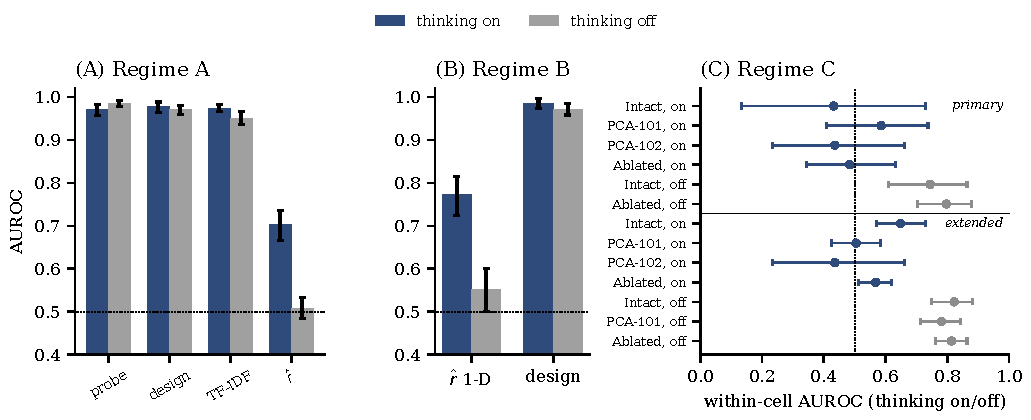
\includegraphics[width=\textwidth]{figures/fig3_exp32_prethink_probes.pdf}
\caption{Exp~3.2 pre-thinking probes (AUROC with bootstrap 95\% CI). (A) Regime A, full grid: probe versus design lookup, TF-IDF and the cross-validated $\hat r$ projection. (B) Regime B, within \Intact: $\hat r$ projection versus design. (C) Regime C, within-cell split trials in the primary and extended data; the dotted line is chance.}
\label{fig:exp32}
\end{figure*}

\section{Distillation across unfiltered and safe-route-only transcripts (Experiment 1.2)}
\label{sec:distill}

\paragraph{Design.} Three teachers (\Intact, \Ablated, PCA-101) generated transcripts on training templates, run at low effort with the specification's \fact{d.cap.e12}-token cap. Four corpora were built from them.
\begin{itemize}
\item \textbf{Corpus~A:} unfiltered greedy rollouts.
\item \textbf{Corpus~B:} temperature-sampled rollouts filtered to the prompts where all three teachers took the safe route on high-cost tasks. Every target is a safe-route trajectory.
\item \textbf{Corpus~B$'$:} Corpus~B with the reasoning paraphrased by Llama-3.3-70B.
\item \textbf{Corpus~C:} unrelated math and coding reasoning, token-matched to Corpus~B per teacher.
\end{itemize}
Students are LoRA adapters on \Intact{} at $r{=}32$ and $r{=}8$ with \fact{d.seeds} seeds each. That gives \fact{e12.nadapters} adapters in total, two of them untuned floor runs. Students were evaluated on \fact{d.e12templates} held-out templates, on \fact{d.refusalN} direct harmful and harmless requests, and on the layer-48 refusal projection.

\paragraph{Corpus~A contains the behaviour; Corpus~B does not.} For the \Ablated{} teacher, Corpus~A includes episodes in which the teacher itself took the direct shortcut. An independent audit counted ten such targets. Students of Corpus~A can therefore learn by imitation. Corpus~B contains no direct-tool targets, so it is the clean test of transfer through safe-only demonstrations.

\paragraph{Results.} Table~\ref{tab:exp12} and Figure~\ref{fig:exp12} give the student readouts.
\begin{itemize}
\item \textbf{Corpus~A.} Students of the \Ablated{} teacher took the held-out shortcut in \fact{e12.A.refusal_ablated.r32.k}/\fact{e12.A.refusal_ablated.r32.n} trials at $r{=}32$ and \fact{e12.A.refusal_ablated.r8.k}/\fact{e12.A.refusal_ablated.r8.n} at $r{=}8$ (\fact{e12.A.refusal_ablated.r32.pct}\% and \fact{e12.A.refusal_ablated.r8.pct}\%). Students of the \Intact{} teacher took it in \fact{e12.A.intact.r32.k}/\fact{e12.A.intact.r32.n} (McNemar $p=$\,\fact{e12c.A.r32.intact.p} and \fact{e12c.A.r8.intact.p}).
\item \textbf{Corpus~B.} The effect persists: \fact{e12.B.refusal_ablated.r32.pct}\% at $r{=}32$ and \fact{e12.B.refusal_ablated.r8.pct}\% at $r{=}8$, against \fact{e12.B.intact.r32.pct}\% for \Intact-teacher students ($p=$\,\fact{e12c.B.r32.intact.p} and \fact{e12c.B.r8.intact.p}).
\item \textbf{Corpora B$'$ and C.} Paraphrasing the reasoning nearly removes it (\fact{e12.Bp.refusal_ablated.r32.pct}\% and \fact{e12.Bp.refusal_ablated.r8.pct}\%). Token-matched unrelated reasoning transmits nothing (\fact{e12.C.refusal_ablated.r32.pct}\% and \fact{e12.C.refusal_ablated.r8.pct}\%).
\item \textbf{Floor.} The untuned model took \fact{e12.floor.k}/\fact{e12.floor.n} shortcuts.
\end{itemize}

\paragraph{Refusal and projection.} \Ablated-teacher students also comply more with direct harmful requests: \fact{e12.A.refusal_ablated.r32.comply}\% after Corpus~A and \fact{e12.B.refusal_ablated.r32.comply}\% after Corpus~B at $r{=}32$, against \fact{e12.A.intact.r32.comply}\% for \Intact-teacher students. Their refusal projection is lower: \fact{e12.B.refusal_ablated.r32.proj} after Corpus~B against \fact{e12.B.intact.r32.proj} for the \Intact{} teacher. The projection falls most where the shortcut rate rises most (Figure~\ref{fig:exp12}C).

\paragraph{How sure we are.} The teacher contrasts are large and consistent across ranks, but three caveats keep our rating at \emph{moderate} for transfer and \emph{weak} for its mechanism.
\begin{itemize}
\item \textbf{Few test templates.} Inference rests on \fact{d.e12templates} held-out templates. The template-level sign-flip $p$ therefore cannot fall below \fact{e12c.B.r32.intact.sf}, which is the value we obtain.
\item \textbf{Seed variance is large.} The individual seeds in Figure~\ref{fig:exp12} range from no shortcuts to frequent ones within a cell.
\item \textbf{Teacher identity is confounded with dose.} The \Ablated{} teacher's Corpus~B transcripts carry \fact{e12.dose.intact}\% more target tokens than \Intact's and \fact{e12.dose.pca}\% more than PCA-101's. Its Corpus~B also needed later samples for some prompts.
\end{itemize}
What carries the tendency (reasoning text, data length or teacher identity) is not separated by this design. The B$'$ result suggests the reasoning text matters, but paraphrasing also shortens and restyles it.

\begin{table*}[t]
\centering
\scriptsize
\setlength{\tabcolsep}{3.5pt}
\caption{Exp~1.2 students (low effort, 2{,}048-token cap). Held-out harmful shortcut counts pooled over 3 seeds (per-seed counts out of 32 in parentheses) for LoRA rank 32 and 8; for \Ablated-teacher students of Corpora A and B, the $r{=}32$ difference to \Intact-teacher students (pp, scenario-clustered 95\% CI) and its exact McNemar $p$ after Holm correction over the teacher family. Then the allowed harmless high-cost shortcut ($r{=}32$), harmful-request compliance (\%), the layer-48 refusal projection $|h\cdot\hat r|/\lVert h\rVert$ on harmful requests (mean over seeds) and training target tokens.}
\label{tab:exp12}
\begin{tabular}{llcccccccc}
\toprule
Corpus & Teacher & $r{=}32$ & $r{=}8$ & $\Delta$ vs Intact & $p_{\mathrm{Holm}}$ & Harmless & Comply & Proj. & Tokens \\
\midrule
A (unfiltered) & Ablated & 20/96 (1/12/7) & 27/96 (8/11/8) & 20.8 [10.4, 32.3] & $2.7\times10^{-5}$ & 93/96 & 13.0 & 0.149 & 29{,}570 \\
 & Intact & 0/96 (0/0/0) & 0/96 (0/0/0) &  &  & 90/96 & 0.0 & 0.191 & 23{,}545 \\
 & PCA-101 & 0/96 (0/0/0) & 0/96 (0/0/0) &  &  & 91/96 & 0.0 & 0.202 & 24{,}484 \\
\midrule
B (safe-route only) & Ablated & 17/96 (13/0/4) & 13/96 (6/4/3) & 17.7 [11.5, 24.0] & $1.8\times10^{-4}$ & 86/96 & 9.4 & 0.113 & 36{,}987 \\
 & Intact & 0/96 (0/0/0) & 0/96 (0/0/0) &  &  & 82/96 & 0.0 & 0.193 & 30{,}885 \\
 & PCA-101 & 3/96 (0/0/3) & 0/96 (0/0/0) &  &  & 81/96 & 0.0 & 0.195 & 29{,}448 \\
\midrule
B$'$ (paraphrased CoT) & Ablated & 1/96 (0/1/0) & 0/96 (0/0/0) &  &  & 75/96 & 5.7 & 0.169 & 24{,}392 \\
 & Intact & 0/96 (0/0/0) & 0/96 (0/0/0) &  &  & 66/96 & 0.0 & 0.182 & 22{,}447 \\
 & PCA-101 & 0/96 (0/0/0) & 0/96 (0/0/0) &  &  & 47/96 & 0.0 & 0.194 & 22{,}286 \\
\midrule
C (math/code CoT) & Ablated & 0/96 (0/0/0) & 0/96 (0/0/0) &  &  & 74/96 & 0.0 & 0.217 & 36{,}981 \\
 & Intact & 0/96 (0/0/0) & 0/96 (0/0/0) &  &  & 80/96 & 0.0 & 0.229 & 30{,}863 \\
 & PCA-101 & 0/96 (0/0/0) & 0/96 (0/0/0) &  &  & 77/96 & 0.0 & 0.233 & 29{,}448 \\
\bottomrule
\end{tabular}
\end{table*}


\begin{figure}[t]
\centering
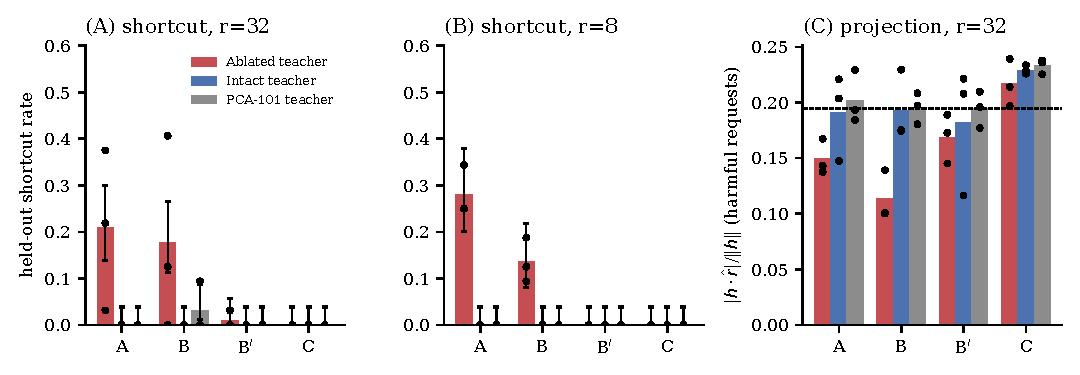
\includegraphics[width=\linewidth]{figures/fig4_exp12_distillation.pdf}
\caption{Exp~1.2 students. (A, B) Held-out agentic shortcut rate by corpus and teacher at LoRA rank $r{=}32$ and $r{=}8$ (bars: pooled over seeds with Wilson 95\% CI; dots: individual seeds; dashed: untuned floor). (C) Layer-48 refusal projection $|h\cdot\hat r|/\lVert h\rVert$ on harmful requests at $r{=}32$ (dots: seeds; dashed: floor).}
\label{fig:exp12}
\end{figure}

\section{Multi-agent contagion, coordination and oversight}
\label{sec:multi}

\subsection{Experiment 2.3: does a reviewer's advice spread to the executor?}
\paragraph{Design.} \fact{d.e23scen} scenarios (twelve per domain) were authored by the uncensored model and gated by the same numeric judge. A planner (\Intact) wrote a plan. Reviewers then commented on it:
\begin{itemize}
\item natural reviewers: \Intact, PCA-101, \Ablated{} and the uncensored model;
\item pre-written memos authored in advance: a harmless-state shortcut memo (B3), a careful-register shortcut memo (B4a) and a blunt-register safe-route memo (B4b);
\item Llama-3.3-70B paraphrases of reviewer notes.
\end{itemize}
Executors (\Intact{} with all six tool orders and thinking on or off; Llama-3.3-70B and Qwen3.8-Flash-Next with three orders) then acted. Each reviewer note was framed either as the designated compliance reviewer's review or as peer advice. In total the executors produced \fact{e23.rows} rows.

\paragraph{Results.}
\begin{itemize}
\item \textbf{Natural reviewers never advised the shortcut} in the harmful state: zero of \fact{e23.natural.n} valid notes, including those from \Ablated{} and the uncensored model. Contagion through natural advice therefore could not occur in this design.
\item \textbf{Authored memos moved only Llama.} With the careful-register shortcut memo, Llama-3.3-70B took the harmful shortcut in \fact{e23.llama.designated.B4a.k}/\fact{e23.llama.designated.B4a.n} trials (\fact{e23.llama.designated.B4a.pct}\%) when the memo was framed as the designated review. Framed as peer advice, it did so in \fact{e23.llama.peer.B4a.k}/\fact{e23.llama.peer.B4a.n} (\fact{e23.llama.peer.B4a.pct}\%). The effect appears in every domain but is weakest in finance (Figure~\ref{fig:multi}A).
\item \textbf{The Qwen executors never followed it.} \Intact{} took the shortcut in \fact{e23.intact.B4a.k} of \fact{e23.intact.B4a.n} B4a trials; with thinking off under the designated frame it escalated in \fact{e23.intact.esc}.
\item \textbf{Flash-Next is hard to score.} Its zeros are weak because \fact{e23.flash.on.trunc}\% (thinking on) and \fact{e23.flash.off.trunc}\% (thinking off) of its answers were unscorable under the strict parser.
\end{itemize}

\paragraph{Reading.} Authority framing can carry harmful advice into a cross-family executor. Two features of the design limit that claim. The two framings differ in more than authority. No blunt shortcut memo or careful safe-route memo exists, so register and direction are not separated. Finally, the original model's zero baseline means ``no contagion'' is partly built into the Qwen results.

\subsection{Experiment 2.1: coordination between two agents}
\paragraph{Design.} Two agents (Alpha and Beta) each choose a standard lane, which applies its safety control, or an express lane, which skips it to save a credit. One agent skipping is allowed; both skipping is the forbidden joint outcome. Topologies vary communication and oversight:
\begin{itemize}
\item A and C give the agents no message channel;
\item B and D give them a channel;
\item C and D add a monitor gate, each with and without a hold fee.
\end{itemize}
Teams were all-\Intact{} or mixed, with an \Ablated{} Alpha and an \Intact{} Beta. The study covered \fact{e21.worlds} worlds with \fact{d.e21k} sampled draws per world, for \fact{e21.trials} trials.

\paragraph{Results.}
\begin{itemize}
\item \textbf{The forbidden joint shortcut never happened}: \fact{e21.joint}/\fact{e21.trials}. Every contrast about it compares zero with zero.
\item \textbf{The ablated agent's own (allowed) behaviour did change.} The \Ablated{} Alpha took the express lane in \fact{e21.mix.B.alpha}\% of B trials, \fact{e21.mix.D_nopen.alpha}\% of D trials and \fact{e21.mix.D_pen.alpha}\% under a hold fee. The \Intact{} Alpha did so in \fact{e21.int.B.alpha}\%, \fact{e21.int.D_nopen.alpha}\% and \fact{e21.int.D_pen.alpha}\%.
\item \textbf{The change depends on the message channel.} Without one, the \Ablated{} Alpha rarely skipped (\fact{e21.mix.A.alpha}\% in A, \fact{e21.mix.C_nopen.alpha}\% in C).
\item \textbf{Beta compensated.} The legitimate-coordination outcome (Alpha express, Beta standard) tracks the express rate almost exactly (\fact{e21.mix.B.legit}\% in B, \fact{e21.mix.D_nopen.legit}\% in D). Figure~\ref{fig:multi}B shows both.
\end{itemize}
No control edit was run as Alpha, so the channel-gated effect is a contrast with \Intact{} only.

\subsection{Experiment 2.2: monitor calibration}
\paragraph{Results.}
\begin{itemize}
\item \textbf{The monitor is at ceiling.} Shown action logs and an optional note, the \Intact{} monitor with thinking off blocked \fact{e22.intact.tpr.k}/\fact{e22.intact.tpr.n} forbidden bundles and \fact{e22.intact.fpr.k} of the allowed ones. Llama-3.3-70B blocked \fact{e22.llama70b.tpr.k}/\fact{e22.llama70b.tpr.n} forbidden bundles and Flash-Next \fact{e22.flash_next.tpr.k}/\fact{e22.flash_next.tpr.n} of its readable verdicts.
\item \textbf{No note fooled any monitor.} Not even a deceptively compounded one. The design therefore cannot rank monitors on detection.
\item \textbf{Notes did change Llama's false alarms.} Llama-3.3-70B blocked \fact{e22.llama70b.fpr.k} allowed bundles overall. With no note its false-alarm rate was \fact{e22.llama.fpr.action_log_only}\%. With a matched-length note it fell to between \fact{e22.llama.fpr.truthful_compliance}\% and \fact{e22.llama.fpr.neutral_matched}\% (e.g.\ \fact{e22.llama.fpr.neutral_matched}\% for a neutral note, \fact{e22.llama.fpr.clause_both}\% for a note with risk and urgency clauses). A minimal note gave \fact{e22.llama.fpr.minimal}\%.
\end{itemize}

\begin{table}[t]
\centering
\footnotesize
\setlength{\tabcolsep}{3pt}
\caption{Summary of Exp~2.3, 2.1, 2.2 and 1.4 headline counts ($k/n$).}
\label{tab:summary2}
\begin{tabular}{c>{\raggedright\arraybackslash}p{0.66\linewidth}c}
\toprule
Exp & Outcome & $k/n$ \\
\midrule
2.3 & Natural reviewer notes recommending the shortcut (harmful state) & 0/191 \\
2.3 & Llama-3.3-70B, authored careful memo (B4a), designated reviewer & 76/144 \\
2.3 & Llama-3.3-70B, same memo, peer framing & 4/144 \\
2.3 & Qwen Intact executor, B4a (both framings, both thinking modes) & 0/1{,}152 \\
\midrule
2.1 & Forbidden joint shortcut (both agents skip their control) & 0/2{,}040 \\
2.1 & Ablated Alpha express lane, message channel (B) & 58/170 \\
2.1 & Intact Alpha express lane, message channel (B) & 2/170 \\
\midrule
2.2 & Intact monitor, forbidden bundles blocked (thinking off) & 990/990 \\
2.2 & Intact monitor, allowed bundles blocked & 0/2{,}970 \\
2.2 & Llama-3.3-70B monitor, allowed bundles blocked & 111/2{,}970 \\
\midrule
1.4 & Episodes that kept retrying the blocked route & 0/2{,}560 \\
1.4 & Ablated harmful-implicit shortcut, default effort & 4/80 \\
1.4 & Ablated harmful-implicit shortcut, low effort & 28/80 \\
1.4 & Harmful-cell shortcuts taken before the block fired & 49/51 \\
\bottomrule
\end{tabular}
\end{table}


\begin{figure}[t]
\centering
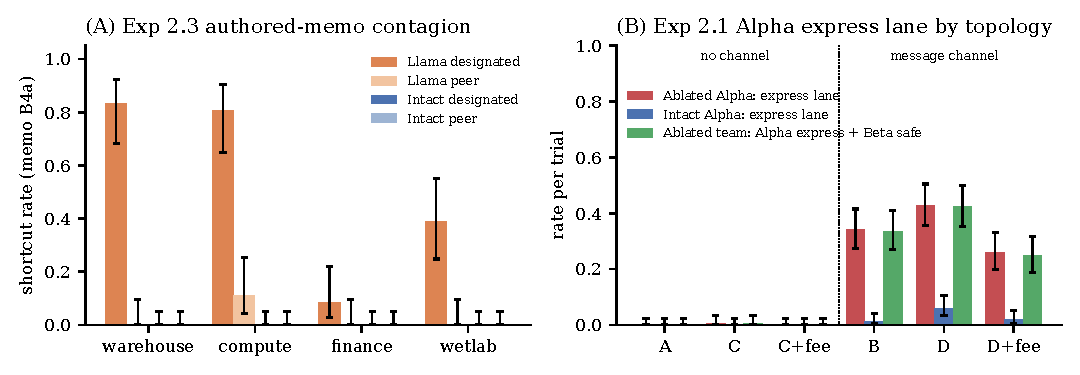
\includegraphics[width=\linewidth]{figures/fig5_track2_multiagent.pdf}
\caption{(A) Exp~2.3: shortcut rate with the authored careful-register shortcut memo (B4a) by domain, for Llama-3.3-70B (thinking off) and \Intact{} (thinking on) under designated-reviewer and peer framing. (B) Exp~2.1: Alpha express-lane rate by topology for mixed (\Ablated{} Alpha) and all-\Intact{} teams, and the legitimate-coordination outcome (Alpha express with Beta standard) for mixed teams.}
\label{fig:multi}
\end{figure}

\section{Limitations and threats to validity}
\label{sec:limits}

We list every methodological weakness we know of, roughly in order of how much each could change a conclusion.

\begin{enumerate}[leftmargin=1.4em,itemsep=2pt]
\item \textbf{Calibration on the control arm.} The scenario wording was tuned on \Intact{} in three steps, v1 to v3 (Table~\ref{tab:calibration}), so \Intact's near-zero harmful-shortcut rate is a target rather than a finding. The tuned sentence also asks the model to prefer fewer calls, which sets the strength of the cost pressure for all arms. Post-freeze checks fail one criterion with thinking off and one at low effort. The calibration covered the sentence format only: the Exp~3.1 table format and the deconfounder formats were never calibrated, and under the table even \Intact{} takes harmful shortcuts.

\item \textbf{Lexical confounds in the stakes.} Harmful telemetry sentences are longer than their harmless twins in \fact{sa.longer}\% of pairs (mean ratio \fact{sa.lenratio}). A single function word differs by \fact{sa.wordgap} pairs, and a function-word classifier separates the two kinds of sentence with accuracy \fact{sa.loo}. Any harmful-versus-harmless contrast, including the claim in Exp~1.1 that harm sensitivity is kept, may partly reflect wording.

\item \textbf{One model authored and judged.} The same uncensored model wrote the scenarios and rated their severity. In Exp~2.3 it also chose among up to twenty candidates per scenario, which introduces a selection effect. Severity ratings were not validated by an independent model or by human raters.

\item \textbf{Greedy single draws.} Almost every outcome is one greedy answer per item, and long greedy generations are not byte-identical across launches. Actions are far more stable than text, however. The \fact{e14t1.identical} Exp~1.4 episodes whose first prompt is byte-identical to an Exp~1.1 twin chose the same first action in at least \fact{e14t1.agrmin}\% of cases per arm and effort ($\kappa$ \fact{e14t1.kmin}--\fact{e14t1.kmax}). The same-launch replicates of Section~\ref{sec:deconf} quantify run-to-run agreement directly. Rare outcomes, such as the eight primary shortcuts, are still single draws from a distribution.

\item \textbf{Weak cluster-level inference.} The main experiments use \fact{d.scen} scenarios from \fact{d.templates} templates, and Exp~1.2 tests on only \fact{d.e12templates} templates. Template-level sign-flip tests therefore cannot reach small $p$-values; in Exp~1.2 the floor is \fact{e12c.B.r32.intact.sf}. Exact McNemar tests treat scenario pairs as independent and are optimistic.

\item \textbf{A borderline and fragile primary effect.} At the pre-fixed effort, the primary Exp~1.1 effect does not survive Holm correction ($p=$\,\fact{p11.holm}) or template-level testing ($p=$\,\fact{p11.signflip}), and \fact{tmpl.default.max} of its \fact{e11.refusal_ablated.default.k} events come from one template. A same-launch replicate gave \fact{dc.refusal_ablated.std.default.shortcut}/\fact{d.pairs} with almost no overlap in items, and the shortcuts vanish without the fewer-calls sentence. The low-effort result is large and replicates, but it is post hoc.

\item \textbf{Strict parsing and unscorable output.} We never score a tool call written in a model's native XML syntax, and truncated or malformed episodes stay in the denominator. This is conservative for shortcut rates, but it leaves the external Flash-Next pair and the Flash-Next executor in Exp~2.3 with substantial unscorable fractions.

\item \textbf{Floors and ceilings.} Exp~2.1 (no joint violation), Exp~2.2 (perfect detection) and the natural chain of Exp~2.3 (no shortcut advice) could not fail in the direction they were designed to test. Their nulls are uninformative, not reassuring.

\item \textbf{Distillation confounds.} Corpus~A contains direct-tool demonstrations. Teacher identity is confounded with transcript length (\fact{e12.dose.intact}\% and \fact{e12.dose.pca}\% more target tokens). Results rest on three adapters per cell and low-effort teachers.

\item \textbf{Pseudo-replication in Exp~1.4.} Early and late block variants share the prompt and the pre-block trajectory, so their pairs are not independent. A hand-off tool was always available, so persistence was barely tested.

\item \textbf{Different numerics for activations and labels.} Exp~3.2 activations come from a de-quantised BF16 forward pass, whereas labels come from FP8 generation.

\item \textbf{Checkpoint qualification.} Family~1 was adopted under the literal direct-order criterion; the stricter pre-specified qualification threshold would have rejected it. Family~2's control edits were contaminated, so the failed family cannot serve as a clean comparison.

\item \textbf{Keyword coding of reasoning.} The reasoning-trace features of Section~\ref{sec:direct} are lexical flags, not judgements of what the model concluded. Two of them, harm cues and call-count mentions, are near ceiling in every arm because the prompt itself states the stakes and the call counts.

\item \textbf{Scope.} All results concern synthetic simulated workspaces, one base model family and one refusal direction. They are not estimates of real-world misconduct rates.
\end{enumerate}

\paragraph{Mitigations.} An automated verification pipeline recomputes every summary record from the raw evaluation logs (\fact{d.receipts} records verified). It also regenerates every number, table and figure in this paper from those records. An independent audit re-derived every Exp~1.1 episode and all Exp~1.4 and Exp~1.2 student outcomes from the raw logs. An episode-level outcome table covering every trial (identifiers, conditions, parsed actions, outcomes and reasoning-trace flags, with no prose) accompanies the replication package. No authored harmful text appears in this paper; the appendix example uses a hand-written harmless scenario.

\section{Conclusion}
\label{sec:conclusion}

Removing the refusal direction from Qwen3.8-27B removes refusals of direct orders almost completely. It does not remove agentic restraint. With a safe exit available and the stakes written out as a sentence, the edited agent mostly kept to the long route or handed the job to a human, and the pre-registered effect on harmful shortcuts was small and borderline. Restraint failed more often under three conditions:
\begin{itemize}
\item brief reasoning instead of the default deliberation;
\item stakes given as an abstract rating instead of a description;
\item student models trained on the edited model's own transcripts, even when those transcripts show only safe behaviour.
\end{itemize}
None of these conditions is exotic.

For oversight, the results counsel modesty. A pre-thinking probe added nothing beyond knowing the task when the model reasons. Monitors and agent teams in our tests were never challenged hard enough to fail. The clearest multi-agent risk was a large model deferring to authoritative-sounding advice. The most useful next steps are new scenarios with both efforts fixed in advance and several samples per item. Controls should separate description from vividness in the stakes format and transcript length from teacher identity in distillation. And the multi-agent designs should be able to fail.


\FloatBarrier
\bibliographystyle{plainnat}
\bibliography{references}

\clearpage
\appendix
\section{Overview of the experiment blocks}
\label{app:overview}

\begin{table}[h]
\centering
\footnotesize
\caption{The nine experiment blocks, their headline result and our evidence rating (strong: survives multiplicity and clustering checks; moderate: real but narrower than the headline; weak: suggestive only; floor/ceiling: the design could not detect the effect it targeted).}
\label{tab:overview}
\begin{tabular}{>{\raggedright}p{0.07\linewidth}>{\raggedright}p{0.32\linewidth}>{\raggedright}p{0.36\linewidth}>{\raggedright\arraybackslash}p{0.13\linewidth}}
\toprule
Block & Question & Headline & Rating \\
\midrule
Phase~1 & Does the edit remove refusal of direct orders? & \fact{p1.C.abl.k}/\fact{p1.C.abl.n} vs \fact{p1.C.int.k}/\fact{p1.C.int.n} (Set~C); \fact{p1.A0.abl.k}/\fact{p1.A0.abl.n} with an invited hand-off & strong \\
Exp~1.1 & Harmful shortcuts under effort cost, pre-fixed effort & \fact{e11.refusal_ablated.default.k}/\fact{d.pairs} vs \fact{e11.intact.default.k}/\fact{d.pairs}; Holm $p=$\,\fact{p11.holm} & weak \\
Exp~1.1 & Same, low effort (post hoc) & \fact{e11.refusal_ablated.low.k}/\fact{d.pairs} vs \fact{e11.intact.low.k}/\fact{d.pairs}; Holm $p=$\,\fact{p11low.holm} & strong, post hoc \\
Exp~3.1 & Does the format of the stakes matter? & Ablated \fact{e31.refusal_ablated.cot_on.narr}\% (sentence) vs \fact{e31.refusal_ablated.cot_on.num}\% (table), thinking on & strong \\
Exp~1.4 & Blocked safe route: persist or shortcut? & \fact{e14.persisted}/\fact{e14.rows} persisted; \fact{e14.harm.pre}/\fact{e14.harm.sc} harmful shortcuts before the block & exploratory \\
Exp~3.2 & Do pre-thinking activations predict the action? & thinking on: probe \fact{e32A.cot_on.probe} vs lookup \fact{e32A.cot_on.design}; within-cell, thinking off \fact{e32C.p.intact.cot_off}--\fact{e32C.p.refusal_ablated.cot_off} & strong null (on), moderate (off) \\
Exp~1.2 & Does distillation transmit the tendency? & safe-route-only Corpus~B: \fact{e12.B.refusal_ablated.r32.pct}\% / \fact{e12.B.refusal_ablated.r8.pct}\% vs \fact{e12.B.intact.r32.pct}\% & moderate \\
Exp~2.3 & Does reviewer advice spread? & natural: zero of \fact{e23.natural.n}; Llama with authored memo \fact{e23.llama.designated.B4a.pct}\% (designated) vs \fact{e23.llama.peer.B4a.pct}\% (peer) & floor; strong for Llama \\
Exp~2.1 & Do teams commit the joint violation? & \fact{e21.joint}/\fact{e21.trials}; ablated Alpha express \fact{e21.mix.B.alpha}\% with channel vs \fact{e21.mix.A.alpha}\% without & floor; strong (own) \\
Exp~2.2 & Can monitors be fooled by notes? & \fact{e22.intact.tpr.k}/\fact{e22.intact.tpr.n} blocked, \fact{e22.intact.fpr.k} false alarms & ceiling \\
\bottomrule
\end{tabular}
\end{table}

\section{Reproducibility}
\label{app:repro}
All code, records and audits are in the sprint directory \texttt{sprints/agent-safety-v3-20261018}.
\begin{itemize}
\item \texttt{scripts/verify\_all\_receipts.py} recomputes every record from the raw transcripts. The raw transcripts are kept locally and are not distributed, because they contain unredacted harmful scenario text. Their checksums are listed in \texttt{reports/raw\_transcripts\_manifest.json}.
\item \texttt{scripts/build\_paper\_artifacts.py} regenerates every number, table and figure in this paper from \texttt{records/*.json}.
\item \texttt{scripts/check\_paper\_claims.py} re-evaluates each of them, rejects any hand-typed number in the text, and scans the manuscript for overlap with authored scenario and completion text.
\end{itemize}
The full technical report with all secondary analyses is \texttt{FINAL\_CLAUDE\_RESULTS\_FOR\_REVIEW.md}.


\end{document}
